% spice2rnm --- product whitepaper
%
% Standard classes and packages only, so this builds with a stock TeX Live
% or MiKTeX and needs no local .sty files:
%   pdflatex spice2rnm-demos.tex   (twice, for the table of contents)
%
% Every figure quoted here is machine-produced by the product itself.
% Regenerate them with:  cd demos && ./run_all.sh
\documentclass[11pt,a4paper]{article}

\usepackage[T1]{fontenc}
\usepackage[utf8]{inputenc}
\usepackage[margin=1in]{geometry}
\usepackage{booktabs}
\usepackage{array}
\usepackage{xcolor}
\usepackage{listings}
\usepackage{amsmath}
\usepackage{enumitem}
\usepackage{fancyhdr}
\usepackage{pgfplots}
\pgfplotsset{compat=1.18}
\usepackage{draftwatermark}
\usepackage[hidelinks]{hyperref}

% Ownership mark on every page. Deliberately faint: at lightness 0.93
% it reads as a mark on the paper rather than as something printed over
% the text, so tables and code listings stay legible on screen and in
% greyscale.
\SetWatermarkText{Veylon Systems}
\SetWatermarkScale{0.32}
\SetWatermarkLightness{0.93}
\SetWatermarkAngle{45}

\definecolor{accent}{HTML}{1F5673}
\definecolor{pass}{HTML}{1B7A3D}
\definecolor{fail}{HTML}{A8322D}
\definecolor{rule}{HTML}{C8CDD2}

\newcommand{\pass}{\textcolor{pass}{\textsc{pass}}}
\newcommand{\unit}[1]{\,\textrm{#1}}

\lstset{
  basicstyle=\ttfamily\footnotesize,
  breaklines=true,
  frame=leftline,
  framerule=1pt,
  rulecolor=\color{rule},
  xleftmargin=1em,
  framexleftmargin=1em,
  aboveskip=1em,
  belowskip=1em,
  showstringspaces=false,
}

\pagestyle{fancy}
\fancyhf{}
\lhead{\footnotesize\textcolor{accent}{Veylon Systems \textperiodcentered{} spice2rnm}}
\rhead{\footnotesize From netlist to verified model}
\cfoot{\thepage}
\renewcommand{\headrulewidth}{0.4pt}

\title{\vspace{-2em}
  {\color{accent}\Huge From netlist to verified model}\\[0.4em]
  {\large Automatic real-number-model and testbench generation\\
   for mixed-signal verification}}
\author{\normalsize Veylon Systems}
\date{}

\begin{document}
\maketitle
\thispagestyle{fancy}
\vspace{-3em}

\begin{abstract}
\noindent
A real number model is a fast stand-in for an analog block. Rather than
solving transistor physics the way SPICE does, it computes an output
number from an input number --- so it runs in an ordinary digital
simulator, alongside the chip's logic, fast enough for a full regression
suite.

The trouble is that somebody has to write it, keep it matching the circuit
as the circuit changes, and convince the team it still matches. The first
two are slow. The third usually never happens at all.

\textbf{spice2rnm} does all three from one command. Give it a SPICE
netlist and you get back a SystemVerilog real number model, a UVM-MS
verification environment that exercises it, and the evidence that both
agree with the real circuit.

Three things make that evidence worth reading. Every expected value in
every generated testbench is a \emph{SPICE measurement of your circuit},
never the model's own equations, so a test cannot pass by agreeing with
itself. Every generated environment is proven able to fail: the tool
breaks the model on purpose and confirms the test goes red. And how a
block gets checked depends on what that block is for --- a filter as a
frequency response, a duty-cycle corrector by where its edges land, a
phase interpolator by how far it moves the clock at each setting.

This paper walks through four circuits, getting harder as it goes. Every
number in it was produced by the shipped tool, in about half an hour on a
laptop.
\end{abstract}

\vspace{0.2em}
\tableofcontents
\vspace{0.2em}

%======================================================================
\section{The problem}

A model of an analog block has to be two things at once, and they pull
against each other. Fast, or it cannot run in a digital regression suite
at all. Accurate, or passing it does not mean anything.

Hand-written models drift away from the circuits they stand for, and the
drift is silent. Nothing breaks. The model still compiles, still
simulates, still passes its tests. It has simply stopped describing the
circuit.

The usual defence is a hand-written testbench, which has the same problem
one level up. A person decides what to check and how close is close
enough, and those decisions are rarely written down beside the numbers
they produced. When the circuit is revised, the model, the testbench and
the tolerances all need revisiting by hand --- which, in practice, is not
what happens.

\textbf{spice2rnm} regenerates all three from the netlist whenever you ask
it to. The model, the environment that checks it, and the evidence trail
all come out of the same command, so they cannot quietly fall out of step
with the circuit or with each other.

%======================================================================
\section{What you get from one command}

\begin{lstlisting}
spice2rnm dcc.cir --input-node clk --output-node vout \
          --emit-uvm-ms --spec dcc_spec.md
\end{lstlisting}

\begin{itemize}[leftmargin=1.5em,itemsep=0.3em]
  \item \textbf{A SystemVerilog real-number model}, with the model
        structure chosen automatically to match the block's measured
        behaviour --- including blocks whose dynamics move with signal
        level, where any fixed-response model is wrong across most of its
        range.

        It presents \texttt{wreal} ports by default, so it wires
        straight into an RNM library like the models beside it. That
        boundary is a module around a computing core, and the core is
        emitted with plain \texttt{real} ports. A \texttt{real} port is a
        \emph{variable}: it depends on no package, no nettype declaration
        and no simulator extension, so the core compiles standalone
        anywhere. A flow without \texttt{wreal} support instantiates it
        directly. The boundary can instead be a user-defined nettype from
        your own library (Section~\ref{sec:style}), or omitted with
        \texttt{-{}-model-ports real}.

        The core is untouched in every case: it is the file the
        equivalence check ran against. A boundary costs nothing in
        fidelity either. Driven with identical stimulus, boundary and
        bare core agree exactly --- worst difference $0$ over $120$
        randomised samples across all three case-study models, and again
        on a library's own nettype. \texttt{wreal} is a simulator extension rather than
        IEEE 1800, so that boundary is a separate file the core does not
        depend on.
  \item \textbf{A UVM-MS verification environment} following the Accellera
        UVM-MS specification, built on IEEE 1800 --- not on Verilog-AMS.
        Analog values travel on \emph{user-defined nettypes} (IEEE
        1800-2017 \S6.6.7) with a generated resolution function. Multiple
        drivers on a net then combine in the net type rather than in
        hand-edited testbench code --- an offset source, a noise
        injector, a second bridge. \texttt{wreal} is a simulator
        extension rather than IEEE 1800, so the generated UVM-MS
        environment drives the core rather than the \texttt{wreal}
        boundary, and needs no AMS licence to run. Bridge and wrapper ports are
        \texttt{interconnect} (\S6.6.8), inheriting the testbench's nettype
        instead of naming one, and scoreboard golden values are SPICE
        measurements of your circuit.
  \item \textbf{Equivalence evidence}: circuit and model driven with the
        identical stimulus, then compared in the domain that matters for
        the block --- waveform error for signal-path blocks, edge
        placement for clock-path blocks. The aligned traces are archived,
        so any verdict can be re-derived from its own run directory.
\end{itemize}

\noindent An optional plain-language functional specification supplies what
no netlist can: the block's intended operating range and its acceptance
criteria (Section~\ref{sec:spec}).

%======================================================================
\section{Case study 1 --- Two-pole filter}

A two-pole RC low-pass filter --- the ordinary case, a block that takes a
signal in and shapes it on the way out. The generated model is checked
four independent ways.

\begin{center}
\begin{tabular}{@{}lr@{}}
\toprule
Chirp equivalence           & $0.0290$ against a $0.15$ threshold \quad \pass \\
PRBS (independent stimulus) & $0.0097$ normalised \quad \pass \\
\midrule
UVM-MS, DC section          & $49$ checks, $0$ failed \\
UVM-MS, AC section          & $15$ checks, $0$ failed \\
\quad worst magnitude       & $0.0674\unit{dB}$ of a $0.25\unit{dB}$ tolerance \\
\quad worst phase           & $2.70^{\circ}$ of an $8.00^{\circ}$ tolerance \\
\bottomrule
\end{tabular}
\end{center}

\noindent The PRBS row matters more than it looks. The model is built from
a chirp --- a tone sweeping upward through frequency --- and then tested
with a pseudo-random bit sequence it has never seen. A model that had
merely memorised the input it was built from would come apart here. This
one does not.

% <<TRACE:lpf2>>
\begin{center}
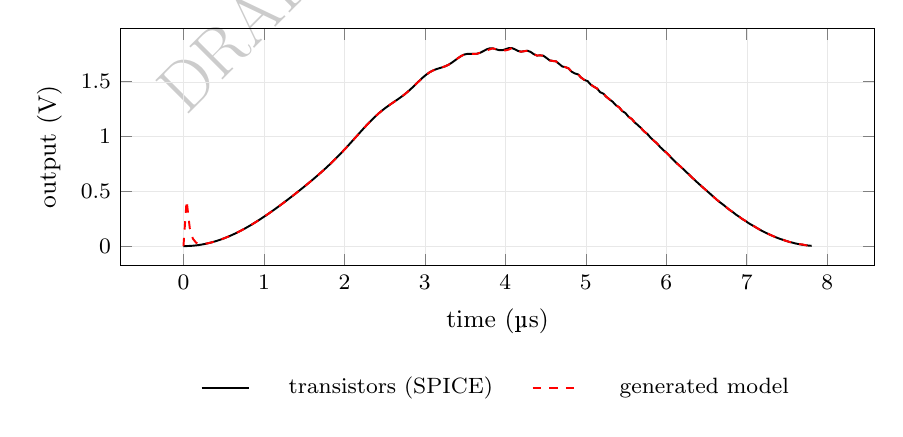
\begin{tikzpicture}
  \begin{axis}[width=0.92\linewidth,height=4.6cm,
    xlabel={time (\textmu s)}, ylabel={output (V)},
    label style={font=\small}, tick label style={font=\footnotesize},
    legend style={font=\footnotesize,at={(0.5,-0.42)},anchor=north,
      legend columns=2,draw=none,column sep=1.2em},
    grid=both, grid style={line width=0.1pt,draw=gray!18},
    every axis plot/.append style={line width=0.7pt}]
    \addplot[black] coordinates {(0,0) (0.03908,0.00030201) (0.078314,0.0014419) (0.11754,0.0034711) (0.15682,0.0064052) (0.19599,0.010231) (0.23525,0.014965) (0.27449,0.020589) (0.31371,0.027096) (0.35295,0.034482) (0.39216,0.042725) (0.43142,0.051833) (0.47066,0.061773) (0.50984,0.072522) (0.54912,0.084104) (0.58833,0.09645) (0.62759,0.10958) (0.66682,0.12344) (0.70601,0.13801) (0.74529,0.15331) (0.7845,0.16924) (0.82372,0.18582) (0.86299,0.20304) (0.90218,0.22079) (0.94147,0.23913) (0.98066,0.25795) (1.0199,0.27726) (1.0592,0.29704) (1.0984,0.3172) (1.1376,0.33777) (1.1768,0.35869) (1.2161,0.37993) (1.2553,0.40151) (1.2945,0.42332) (1.3338,0.44545) (1.373,0.46782) (1.4122,0.49045) (1.4515,0.51335) (1.4907,0.53651) (1.5299,0.56) (1.5692,0.5838) (1.6084,0.60793) (1.6476,0.63254) (1.6868,0.65756) (1.7261,0.68314) (1.7653,0.70928) (1.8045,0.73602) (1.8438,0.76352) (1.883,0.7917) (1.9222,0.82063) (1.9615,0.85036) (2.0007,0.88075) (2.04,0.91186) (2.0792,0.94345) (2.1184,0.97545) (2.1577,1.0077) (2.1969,1.0398) (2.2361,1.0716) (2.2754,1.1028) (2.3146,1.1329) (2.3539,1.1619) (2.393,1.1893) (2.4323,1.2151) (2.4715,1.2391) (2.5107,1.2615) (2.55,1.2824) (2.5892,1.3024) (2.6285,1.3219) (2.6677,1.3415) (2.7069,1.362) (2.7462,1.3839) (2.7854,1.4075) (2.8246,1.4331) (2.8639,1.4604) (2.9031,1.4885) (2.9423,1.5165) (2.9815,1.543) (3.0208,1.5667) (3.06,1.5866) (3.0992,1.6022) (3.1385,1.614) (3.1777,1.6232) (3.2169,1.6318) (3.2562,1.6421) (3.2954,1.6558) (3.3346,1.6737) (3.3739,1.6948) (3.4131,1.7166) (3.4524,1.7356) (3.4915,1.7487) (3.5308,1.7547) (3.57,1.755) (3.6093,1.7538) (3.6485,1.7559) (3.6877,1.7647) (3.727,1.7794) (3.7662,1.795) (3.8054,1.8048) (3.8447,1.8047) (3.8839,1.7966) (3.9232,1.7883) (3.9624,1.7877) (4.0016,1.7963) (4.0409,1.8065) (4.0801,1.8076) (4.1193,1.7961) (4.1586,1.7807) (4.1977,1.7744) (4.237,1.7795) (4.2762,1.783) (4.3154,1.7719) (4.3547,1.7511) (4.3939,1.739) (4.4332,1.7406) (4.4724,1.7376) (4.5116,1.7171) (4.5509,1.695) (4.5901,1.6898) (4.6293,1.6861) (4.6686,1.6632) (4.7078,1.639) (4.747,1.6334) (4.7862,1.6215) (4.8255,1.5915) (4.8647,1.5755) (4.9039,1.5672) (4.9432,1.5374) (4.9824,1.5162) (5.0217,1.5062) (5.0609,1.4741) (5.1001,1.4549) (5.1394,1.4387) (5.1786,1.4047) (5.2178,1.3916) (5.2571,1.3613) (5.2963,1.338) (5.3355,1.3164) (5.3747,1.2848) (5.414,1.2671) (5.4532,1.2325) (5.4924,1.2147) (5.5317,1.1798) (5.5709,1.1603) (5.6101,1.1271) (5.6494,1.1032) (5.6886,1.0754) (5.7279,1.044) (5.7671,1.0224) (5.8063,0.98828) (5.8456,0.96206) (5.8848,0.93745) (5.924,0.90414) (5.9633,0.87607) (6.0024,0.85212) (6.0417,0.82302) (6.0809,0.7915) (6.1202,0.76301) (6.1594,0.73729) (6.1986,0.71154) (6.2379,0.68448) (6.2771,0.65674) (6.3163,0.62903) (6.3556,0.60178) (6.3948,0.5752) (6.4341,0.54924) (6.4733,0.52387) (6.5125,0.49875) (6.5518,0.47332) (6.591,0.4474) (6.6302,0.42187) (6.6694,0.39886) (6.7087,0.37748) (6.7479,0.35355) (6.7871,0.33039) (6.8264,0.31088) (6.8656,0.28784) (6.9048,0.26905) (6.9441,0.24773) (6.9833,0.23025) (7.0225,0.21006) (7.0618,0.1931) (7.101,0.17667) (7.1402,0.15933) (7.1794,0.14314) (7.2187,0.12834) (7.2579,0.11439) (7.2971,0.10107) (7.3364,0.088309) (7.3756,0.076398) (7.4148,0.065725) (7.4541,0.056208) (7.4933,0.046483) (7.5326,0.037644) (7.5718,0.030667) (7.611,0.023244) (7.6503,0.017643) (7.6895,0.01287) (7.7287,0.0082839) (7.768,0.0048077) (7.8072,0.0023974)};
    \addplot[red,dashed] coordinates {(0,0) (0.03908,0.41726) (0.078314,0.1642) (0.11754,0.066802) (0.15682,0.030984) (0.19599,0.019791) (0.23525,0.018652) (0.27449,0.021971) (0.31371,0.027582) (0.35295,0.034623) (0.39216,0.042732) (0.43142,0.051753) (0.47066,0.061648) (0.50984,0.072387) (0.54912,0.083982) (0.58833,0.096334) (0.62759,0.10942) (0.66682,0.12325) (0.70601,0.13782) (0.74529,0.15315) (0.7845,0.16909) (0.82372,0.18568) (0.86299,0.2028) (0.90218,0.22056) (0.94147,0.23893) (0.98066,0.25776) (1.0199,0.27709) (1.0592,0.29676) (1.0984,0.31694) (1.1376,0.33754) (1.1768,0.35848) (1.2161,0.37976) (1.2553,0.40121) (1.2945,0.42303) (1.3338,0.4452) (1.373,0.4676) (1.4122,0.49026) (1.4515,0.51305) (1.4907,0.5362) (1.5299,0.55973) (1.5692,0.58356) (1.6084,0.60771) (1.6476,0.63237) (1.6868,0.65722) (1.7261,0.68284) (1.7653,0.70901) (1.8045,0.73577) (1.8438,0.76332) (1.883,0.79131) (1.9222,0.82026) (1.9615,0.85005) (2.0007,0.88046) (2.04,0.91163) (2.0792,0.94301) (2.1184,0.97505) (2.1577,1.0074) (2.1969,1.0395) (2.2361,1.0714) (2.2754,1.1026) (2.3146,1.1326) (2.3539,1.1616) (2.393,1.189) (2.4323,1.2149) (2.4715,1.2389) (2.5107,1.2612) (2.55,1.2822) (2.5892,1.3022) (2.6285,1.3217) (2.6677,1.3414) (2.7069,1.3617) (2.7462,1.3836) (2.7854,1.4073) (2.8246,1.4329) (2.8639,1.4602) (2.9031,1.4881) (2.9423,1.5162) (2.9815,1.5427) (3.0208,1.5665) (3.06,1.5865) (3.0992,1.6021) (3.1385,1.6139) (3.1777,1.6231) (3.2169,1.6317) (3.2562,1.642) (3.2954,1.6557) (3.3346,1.6734) (3.3739,1.6946) (3.4131,1.7164) (3.4524,1.7355) (3.4915,1.7486) (3.5308,1.7547) (3.57,1.755) (3.6093,1.7538) (3.6485,1.7559) (3.6877,1.7646) (3.727,1.7792) (3.7662,1.7841) (3.8054,1.7954) (3.8447,1.8047) (3.8839,1.7967) (3.9232,1.7883) (3.9624,1.7877) (4.0016,1.7859) (4.0409,1.7928) (4.0801,1.8077) (4.1193,1.7962) (4.1586,1.7808) (4.1977,1.7744) (4.237,1.7794) (4.2762,1.783) (4.3154,1.772) (4.3547,1.7513) (4.3939,1.7391) (4.4332,1.7406) (4.4724,1.7377) (4.5116,1.7173) (4.5509,1.6952) (4.5901,1.6898) (4.6293,1.6862) (4.6686,1.6634) (4.7078,1.6392) (4.747,1.6334) (4.7862,1.6218) (4.8255,1.5918) (4.8647,1.5756) (4.9039,1.5674) (4.9432,1.5377) (4.9824,1.5163) (5.0217,1.5064) (5.0609,1.4744) (5.1001,1.455) (5.1394,1.439) (5.1786,1.405) (5.2178,1.3917) (5.2571,1.3616) (5.2963,1.338) (5.3355,1.3168) (5.3747,1.285) (5.414,1.2674) (5.4532,1.2326) (5.4924,1.215) (5.5317,1.18) (5.5709,1.1607) (5.6101,1.1273) (5.6494,1.1036) (5.6886,1.0755) (5.7279,1.0444) (5.7671,1.0227) (5.8063,0.98847) (5.8456,0.96241) (5.8848,0.93764) (5.924,0.90432) (5.9633,0.87653) (6.0024,0.8525) (6.0417,0.82316) (6.0809,0.79165) (6.1202,0.76337) (6.1594,0.73777) (6.1986,0.71193) (6.2379,0.68472) (6.2771,0.65691) (6.3163,0.62918) (6.3556,0.60196) (6.3948,0.57537) (6.4341,0.54938) (6.4733,0.52401) (6.5125,0.49897) (6.5518,0.4737) (6.591,0.44779) (6.6302,0.42213) (6.6694,0.39898) (6.7087,0.37766) (6.7479,0.35396) (6.7871,0.33059) (6.8264,0.31106) (6.8656,0.28807) (6.9048,0.26918) (6.9441,0.24803) (6.9833,0.23044) (7.0225,0.21021) (7.0618,0.19333) (7.101,0.17679) (7.1402,0.15943) (7.1794,0.14331) (7.2187,0.12853) (7.2579,0.11457) (7.2971,0.10125) (7.3364,0.088517) (7.3756,0.076543) (7.4148,0.06577) (7.4541,0.056263) (7.4933,0.046625) (7.5326,0.037687) (7.5718,0.030784) (7.611,0.02327) (7.6503,0.017744) (7.6895,0.015491) (7.7287,0.0082696) (7.768,0.0048206) (7.8072,0.002428)};
    \legend{transistors (SPICE), generated model}
  \end{axis}
\end{tikzpicture}
\end{center}
\vspace{-0.6em}
\noindent{\footnotesize The model against the transistors over the whole transient. The two traces are drawn from \texttt{waveform\_compare.csv} in that run's own \texttt{equivalence/} directory.}\vspace{0.6em}
% <<END TRACE:lpf2>>

%======================================================================
\section{Case study 2 --- Duty-cycle corrector}
\label{sec:dcc}

A duty-cycle corrector built around a comparator. How fast it responds is
not fixed: it changes by a factor of $613{,}666$ depending on the input
level. A model with one fixed response cannot represent that at all, and
the standard AC-based way of checking such a model does not work either.
That combination is why blocks like this tend to have the hand-written
models people trust least.

\subsection{A model that follows the circuit's dynamics}

spice2rnm notices that level dependence while it is measuring the circuit,
and builds a model whose speed varies with level the way the measurements
say it should. That includes the circuit's rise/fall asymmetry --- it takes
longer to switch one way than the other, by a measured $95\unit{ps}$ ---
which the model reproduces. Fed a clock that is high exactly half the
time, the model's output duty matches the circuit's to $0.000$ percentage
points.

\begin{center}
\begin{tabular}{@{}lr@{}}
\toprule
Transient equivalence   & $0.0769$ against a $0.15$ threshold \quad \pass \\
UVM-MS, DC section      & $46$ checks, $0$ failed \\
UVM-MS, duty section    & $14$ checks, $0$ failed \\
\quad worst duty error  & $0.313$ pp of a $0.500$ pp tolerance \\
\bottomrule
\end{tabular}
\end{center}

\subsection{Verified by function, not by formula}

The testbench generated for this block has \emph{no AC section}, and that
is a measured decision rather than an oversight. An AC sweep assumes the
circuit sits at one operating point and wiggles gently around it. A
comparator in normal use never does that --- it slams between two states.
Check this model that way and it fails every single point by more than
$55\unit{dB}$, despite being demonstrably accurate. The failure tells you
nothing about the model and everything about using the wrong check.

So the environment checks what a duty-cycle corrector is actually for. The
tool drives the real circuit with clocks at several rates and several input
duties, records what duty comes back out of SPICE each time, and holds the
model to those recorded answers. The table spans $20$ percentage points of
measured behaviour --- wide enough that a model ignoring its input could
not fake its way through.

% <<TRACE:dcc2>>
\begin{center}
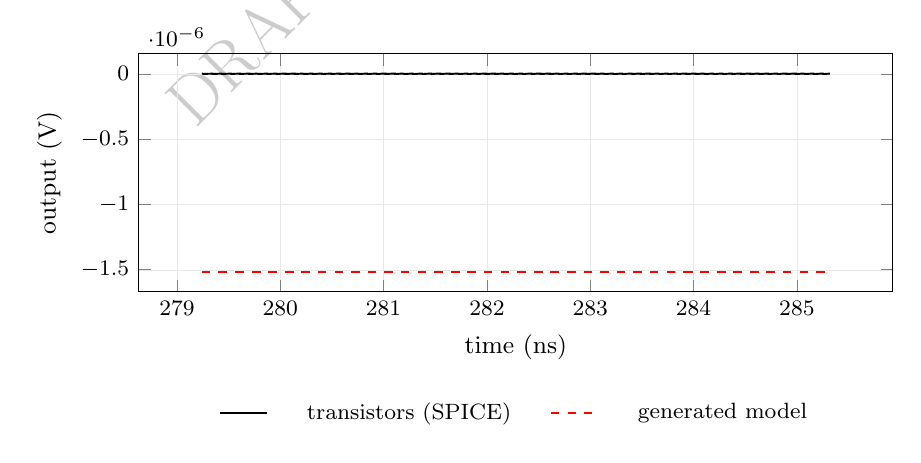
\begin{tikzpicture}
  \begin{axis}[width=0.92\linewidth,height=4.6cm,
    xlabel={time (ns)}, ylabel={output (V)},
    label style={font=\small}, tick label style={font=\footnotesize},
    legend style={font=\footnotesize,at={(0.5,-0.42)},anchor=north,
      legend columns=2,draw=none,column sep=1.2em},
    grid=both, grid style={line width=0.1pt,draw=gray!18},
    every axis plot/.append style={line width=0.7pt}]
    \addplot[black] coordinates {(279.24,9.7209e-10) (279.25,9.5827e-10) (279.26,1.9433e-10) (279.26,-7.945e-10) (279.27,-9.7468e-10) (279.29,8.0331e-11) (279.31,8.6152e-10) (279.33,9.8243e-10) (279.34,9.6811e-10) (279.34,1.9832e-10) (279.35,-7.9803e-10) (279.36,-9.7968e-10) (279.38,8.2527e-11) (279.4,8.6861e-10) (279.41,9.8997e-10) (279.43,9.7519e-10) (279.43,1.969e-10) (279.44,-8.1036e-10) (279.45,-9.9376e-10) (279.46,8.0199e-11) (279.49,8.7488e-10) (279.5,9.9772e-10) (279.52,9.8296e-10) (279.52,1.9298e-10) (279.53,-8.2925e-10) (279.53,-1.0149e-09) (279.55,7.5737e-11) (279.57,8.8275e-10) (279.59,1.0078e-09) (279.61,9.9317e-10) (279.61,1.9472e-10) (279.61,-8.3837e-10) (279.62,-1.0258e-09) (279.64,7.6178e-11) (279.66,8.9119e-10) (279.68,1.0173e-09) (279.7,1.0023e-09) (279.7,1.981e-10) (279.7,-8.4241e-10) (279.71,-1.0312e-09) (279.73,7.8016e-11) (279.75,8.9795e-10) (279.77,1.0246e-09) (279.78,1.0092e-09) (279.79,1.9654e-10) (279.79,-8.5477e-10) (279.8,-1.0453e-09) (279.82,7.5656e-11) (279.84,9.0412e-10) (279.86,1.0322e-09) (279.87,1.0169e-09) (279.87,1.9259e-10) (279.88,-8.7361e-10) (279.89,-1.0663e-09) (279.9,7.123e-11) (279.93,9.1193e-10) (279.94,1.0423e-09) (279.96,1.0271e-09) (279.96,1.9428e-10) (279.97,-8.8277e-10) (279.98,-1.0772e-09) (279.99,7.1666e-11) (280.01,9.2035e-10) (280.03,1.0517e-09) (280.05,1.0362e-09) (280.05,2.0086e-10) (280.05,-8.7948e-10) (280.06,-1.0747e-09) (280.08,7.6453e-11) (280.1,9.2618e-10) (280.12,1.0572e-09) (280.14,1.0411e-09) (280.14,1.9414e-10) (280.14,-9.0104e-10) (280.15,-1.0984e-09) (280.17,6.9601e-11) (280.19,9.3196e-10) (280.21,1.0656e-09) (280.22,1.0499e-09) (280.23,1.917e-10) (280.23,-9.1788e-10) (280.24,-1.1173e-09) (280.26,6.6664e-11) (280.28,9.406e-10) (280.3,1.0762e-09) (280.31,1.0605e-09) (280.31,2.0246e-10) (280.32,-9.0684e-10) (280.33,-1.1066e-09) (280.35,7.5231e-11) (280.37,9.4662e-10) (280.38,1.0809e-09) (280.4,1.0643e-09) (280.4,1.9206e-10) (280.41,-9.3543e-10) (280.42,-1.1377e-09) (280.43,6.5042e-11) (280.46,9.5234e-10) (280.47,1.0901e-09) (280.49,1.0742e-09) (280.49,1.9931e-10) (280.5,-9.3153e-10) (280.5,-1.1344e-09) (280.52,7.0928e-11) (280.54,9.5929e-10) (280.56,1.0966e-09) (280.58,1.08e-09) (280.58,1.9381e-10) (280.58,-9.514e-10) (280.59,-1.1563e-09) (280.61,6.506e-11) (280.63,9.654e-10) (280.65,1.105e-09) (280.67,1.0888e-09) (280.67,1.9706e-10) (280.67,-9.5526e-10) (280.68,-1.1613e-09) (280.7,6.7284e-11) (280.72,9.7234e-10) (280.74,1.1124e-09) (280.75,1.0959e-09) (280.76,1.9582e-10) (280.76,-9.6703e-10) (280.77,-1.1746e-09) (280.79,6.5292e-11) (280.81,9.7851e-10) (280.83,1.12e-09) (280.84,1.1035e-09) (280.84,2.0079e-10) (280.85,-9.6538e-10) (280.86,-1.1735e-09) (280.87,6.9059e-11) (280.9,9.8365e-10) (280.91,1.125e-09) (280.93,1.108e-09) (280.93,1.9118e-10) (280.94,-9.9304e-10) (280.95,-1.2036e-09) (280.96,5.9836e-11) (280.98,9.9007e-10) (281,1.1347e-09) (281.02,1.1184e-09) (281.02,2.0213e-10) (281.02,-9.8127e-10) (281.03,-1.1919e-09) (281.05,6.8991e-11) (281.07,9.9627e-10) (281.09,1.1396e-09) (281.11,1.1223e-09) (281.11,1.9747e-10) (281.11,-9.9677e-10) (281.12,-1.2089e-09) (281.14,6.4069e-11) (281.16,1.0003e-09) (281.18,1.1455e-09) (281.19,1.1286e-09) (281.2,1.9573e-10) (281.2,-1.0088e-09) (281.21,-1.2221e-09) (281.23,6.2177e-11) (281.25,1.0065e-09) (281.27,1.1531e-09) (281.28,1.1363e-09) (281.28,1.9788e-10) (281.29,-1.0136e-09) (281.3,-1.228e-09) (281.32,6.3439e-11) (281.34,1.0125e-09) (281.35,1.1597e-09) (281.37,1.1427e-09) (281.37,1.9908e-10) (281.38,-1.0189e-09) (281.39,-1.2342e-09) (281.4,6.3876e-11) (281.43,1.0175e-09) (281.44,1.1654e-09) (281.46,1.1482e-09) (281.46,1.9621e-10) (281.47,-1.0325e-09) (281.47,-1.2491e-09) (281.49,6.0842e-11) (281.51,1.023e-09) (281.53,1.1725e-09) (281.55,1.1556e-09) (281.55,2.0135e-10) (281.55,-1.03e-09) (281.56,-1.2471e-09) (281.58,6.4931e-11) (281.6,1.0279e-09) (281.62,1.1772e-09) (281.64,1.1598e-09) (281.64,2.0013e-10) (281.64,-1.0381e-09) (281.65,-1.256e-09) (281.67,6.3386e-11) (281.69,1.0316e-09) (281.71,1.1819e-09) (281.72,1.1647e-09) (281.73,1.97e-10) (281.73,-1.0513e-09) (281.74,-1.2704e-09) (281.76,6.0368e-11) (281.78,1.0367e-09) (281.8,1.1886e-09) (281.81,1.1716e-09) (281.81,1.9852e-10) (281.82,-1.0566e-09) (281.83,-1.2765e-09) (281.84,6.1297e-11) (281.87,1.0424e-09) (281.88,1.1949e-09) (281.9,1.1777e-09) (281.9,2.0242e-10) (281.91,-1.0554e-09) (281.92,-1.2757e-09) (281.93,6.4272e-11) (281.95,1.0463e-09) (281.97,1.1988e-09) (281.99,1.1814e-09) (281.99,2.0097e-10) (281.99,-1.0633e-09) (282,-1.2842e-09) (282.02,6.2717e-11) (282.04,1.0497e-09) (282.06,1.2032e-09) (282.08,1.1859e-09) (282.08,1.9721e-10) (282.08,-1.0774e-09) (282.09,-1.2995e-09) (282.11,5.9238e-11) (282.13,1.0547e-09) (282.15,1.2099e-09) (282.16,1.1929e-09) (282.17,2.0216e-10) (282.17,-1.075e-09) (282.18,-1.2974e-09) (282.2,6.3289e-11) (282.22,1.0594e-09) (282.24,1.2144e-09) (282.25,1.197e-09) (282.25,2.0382e-10) (282.26,-1.0763e-09) (282.27,-1.299e-09) (282.29,6.4414e-11) (282.31,1.0621e-09) (282.32,1.2173e-09) (282.34,1.2e-09) (282.34,1.9894e-10) (282.35,-1.091e-09) (282.36,-1.3146e-09) (282.37,6.0055e-11) (282.4,1.066e-09) (282.41,1.2229e-09) (282.43,1.206e-09) (282.43,2.0556e-10) (282.44,-1.0835e-09) (282.44,-1.3069e-09) (282.46,6.5784e-11) (282.48,1.0694e-09) (282.5,1.2256e-09) (282.52,1.2082e-09) (282.52,1.9995e-10) (282.52,-1.0989e-09) (282.53,-1.3233e-09) (282.55,6.0662e-11) (282.57,1.0726e-09) (282.59,1.2306e-09) (282.61,1.2138e-09) (282.61,2.032e-10) (282.61,-1.0985e-09) (282.62,-1.323e-09) (282.64,6.3532e-11) (282.66,1.0766e-09) (282.68,1.2347e-09) (282.69,1.2177e-09) (282.7,2.0222e-10) (282.7,-1.1055e-09) (282.71,-1.3306e-09) (282.73,6.2462e-11) (282.75,1.08e-09) (282.77,1.239e-09) (282.78,1.2222e-09) (282.78,2.0728e-10) (282.79,-1.0995e-09) (282.8,-1.3243e-09) (282.81,6.688e-11) (282.84,1.0823e-09) (282.85,1.2408e-09) (282.87,1.2236e-09) (282.87,2.0396e-10) (282.88,-1.1087e-09) (282.89,-1.3339e-09) (282.9,6.4003e-11) (282.92,1.0843e-09) (282.94,1.2439e-09) (282.96,1.2272e-09) (282.96,2.0232e-10) (282.96,-1.1167e-09) (282.97,-1.3424e-09) (282.99,6.2749e-11) (283.01,1.0879e-09) (283.03,1.2485e-09) (283.05,1.232e-09) (283.05,2.081e-10) (283.05,-1.1095e-09) (283.06,-1.3348e-09) (283.08,6.7786e-11) (283.1,1.0903e-09) (283.12,1.2502e-09) (283.13,1.2334e-09) (283.14,2.0467e-10) (283.14,-1.1189e-09) (283.15,-1.3446e-09) (283.17,6.4822e-11) (283.19,1.0922e-09) (283.21,1.2533e-09) (283.22,1.2369e-09) (283.22,2.0888e-10) (283.23,-1.1136e-09) (283.24,-1.3388e-09) (283.26,6.8746e-11) (283.28,1.0941e-09) (283.29,1.2547e-09) (283.31,1.2381e-09) (283.31,2.054e-10) (283.32,-1.1228e-09) (283.33,-1.3483e-09) (283.34,6.5856e-11) (283.37,1.0958e-09) (283.38,1.2576e-09) (283.4,1.2415e-09) (283.4,2.0664e-10) (283.41,-1.1241e-09) (283.41,-1.3496e-09) (283.43,6.7195e-11) (283.45,1.0985e-09) (283.47,1.2605e-09) (283.49,1.2445e-09) (283.49,2.1075e-10) (283.49,-1.1183e-09) (283.5,-1.3433e-09) (283.52,7.0892e-11) (283.54,1.0996e-09) (283.56,1.2612e-09) (283.58,1.245e-09) (283.58,2.0622e-10) (283.58,-1.129e-09) (283.59,-1.3542e-09) (283.61,6.7219e-11) (283.63,1.1011e-09) (283.65,1.264e-09) (283.66,1.2485e-09) (283.67,2.1087e-10) (283.67,-1.1226e-09) (283.68,-1.3472e-09) (283.7,7.1613e-11) (283.72,1.1029e-09) (283.73,1.2651e-09) (283.75,1.2494e-09) (283.75,2.1253e-10) (283.76,-1.1197e-09) (283.77,-1.3438e-09) (283.78,7.3275e-11) (283.81,1.1028e-09) (283.82,1.2649e-09) (283.84,1.2493e-09) (283.84,2.0795e-10) (283.85,-1.1297e-09) (283.86,-1.3539e-09) (283.87,6.9769e-11) (283.89,1.1039e-09) (283.91,1.2673e-09) (283.93,1.2523e-09) (283.93,2.1177e-10) (283.93,-1.1246e-09) (283.94,-1.3482e-09) (283.96,7.3499e-11) (283.98,1.1055e-09) (284,1.2684e-09) (284.02,1.2534e-09) (284.02,2.1394e-10) (284.02,-1.1207e-09) (284.03,-1.3437e-09) (284.05,7.5645e-11) (284.07,1.1054e-09) (284.09,1.2681e-09) (284.1,1.2531e-09) (284.11,2.1203e-10) (284.11,-1.1245e-09) (284.12,-1.3471e-09) (284.14,7.4486e-11) (284.16,1.1056e-09) (284.18,1.2688e-09) (284.19,1.2543e-09) (284.19,2.1408e-10) (284.2,-1.121e-09) (284.21,-1.3429e-09) (284.23,7.6779e-11) (284.25,1.1059e-09) (284.26,1.269e-09) (284.28,1.2546e-09) (284.28,2.128e-10) (284.29,-1.124e-09) (284.3,-1.3455e-09) (284.31,7.6127e-11) (284.34,1.1063e-09) (284.35,1.2699e-09) (284.37,1.2558e-09) (284.37,2.1782e-10) (284.38,-1.1139e-09) (284.38,-1.3343e-09) (284.4,8.0968e-11) (284.42,1.1058e-09) (284.44,1.2684e-09) (284.46,1.2543e-09) (284.46,2.1481e-10) (284.46,-1.1185e-09) (284.47,-1.3385e-09) (284.49,7.8893e-11) (284.51,1.105e-09) (284.53,1.2683e-09) (284.55,1.2548e-09) (284.55,2.1624e-10) (284.55,-1.1155e-09) (284.56,-1.3347e-09) (284.58,8.0807e-11) (284.6,1.1051e-09) (284.62,1.2682e-09) (284.63,1.2549e-09) (284.64,2.2058e-10) (284.64,-1.1054e-09) (284.65,-1.3234e-09) (284.67,8.506e-11) (284.69,1.1036e-09) (284.7,1.2657e-09) (284.72,1.2525e-09) (284.72,2.1628e-10) (284.73,-1.1118e-09) (284.74,-1.3293e-09) (284.75,8.2028e-11) (284.78,1.1025e-09) (284.79,1.2656e-09) (284.81,1.253e-09) (284.81,2.1829e-10) (284.82,-1.1076e-09) (284.83,-1.3242e-09) (284.84,8.4498e-11) (284.86,1.1024e-09) (284.88,1.2652e-09) (284.9,1.2528e-09) (284.9,2.2188e-10) (284.9,-1.0988e-09) (284.91,-1.3143e-09) (284.93,8.8114e-11) (284.95,1.1008e-09) (284.97,1.2628e-09) (284.99,1.2506e-09) (284.99,2.182e-10) (284.99,-1.104e-09) (285,-1.3189e-09) (285.02,8.5655e-11) (285.04,1.0997e-09) (285.06,1.2625e-09) (285.07,1.251e-09) (285.08,2.2853e-10) (285.08,-1.0807e-09) (285.09,-1.2935e-09) (285.11,9.5236e-11) (285.13,1.0969e-09) (285.15,1.2573e-09) (285.16,1.2454e-09) (285.16,2.1542e-10) (285.17,-1.103e-09) (285.18,-1.3159e-09) (285.2,8.4777e-11) (285.22,1.0954e-09) (285.23,1.2585e-09) (285.25,1.2481e-09) (285.25,2.2826e-10) (285.26,-1.0769e-09) (285.27,-1.2878e-09) (285.28,9.6666e-11) (285.31,1.0943e-09) (285.32,1.2547e-09)};
    \addplot[red,dashed] coordinates {(279.24,-1.5151e-06) (279.25,-1.5151e-06) (279.26,-1.5151e-06) (279.26,-1.5151e-06) (279.27,-1.5151e-06) (279.29,-1.5151e-06) (279.31,-1.5151e-06) (279.33,-1.5151e-06) (279.34,-1.5151e-06) (279.34,-1.5151e-06) (279.35,-1.5151e-06) (279.36,-1.5151e-06) (279.38,-1.5151e-06) (279.4,-1.5151e-06) (279.41,-1.5151e-06) (279.43,-1.5151e-06) (279.43,-1.5151e-06) (279.44,-1.5151e-06) (279.45,-1.5151e-06) (279.46,-1.5151e-06) (279.49,-1.5151e-06) (279.5,-1.5151e-06) (279.52,-1.5151e-06) (279.52,-1.5151e-06) (279.53,-1.5151e-06) (279.53,-1.5151e-06) (279.55,-1.5151e-06) (279.57,-1.5151e-06) (279.59,-1.5151e-06) (279.61,-1.5151e-06) (279.61,-1.5151e-06) (279.61,-1.5151e-06) (279.62,-1.5151e-06) (279.64,-1.5151e-06) (279.66,-1.5151e-06) (279.68,-1.5151e-06) (279.7,-1.5151e-06) (279.7,-1.5151e-06) (279.7,-1.5151e-06) (279.71,-1.5151e-06) (279.73,-1.5151e-06) (279.75,-1.5151e-06) (279.77,-1.5151e-06) (279.78,-1.5151e-06) (279.79,-1.5151e-06) (279.79,-1.5151e-06) (279.8,-1.5151e-06) (279.82,-1.5151e-06) (279.84,-1.5151e-06) (279.86,-1.5151e-06) (279.87,-1.5151e-06) (279.87,-1.5151e-06) (279.88,-1.5151e-06) (279.89,-1.5151e-06) (279.9,-1.5151e-06) (279.93,-1.5151e-06) (279.94,-1.5151e-06) (279.96,-1.5151e-06) (279.96,-1.5151e-06) (279.97,-1.5151e-06) (279.98,-1.5151e-06) (279.99,-1.5151e-06) (280.01,-1.5151e-06) (280.03,-1.5151e-06) (280.05,-1.5151e-06) (280.05,-1.5151e-06) (280.05,-1.5151e-06) (280.06,-1.5151e-06) (280.08,-1.5151e-06) (280.1,-1.5151e-06) (280.12,-1.5151e-06) (280.14,-1.5151e-06) (280.14,-1.5151e-06) (280.14,-1.5151e-06) (280.15,-1.5151e-06) (280.17,-1.5151e-06) (280.19,-1.5151e-06) (280.21,-1.5151e-06) (280.22,-1.5151e-06) (280.23,-1.5151e-06) (280.23,-1.5151e-06) (280.24,-1.5151e-06) (280.26,-1.5151e-06) (280.28,-1.5151e-06) (280.3,-1.5151e-06) (280.31,-1.5151e-06) (280.31,-1.5151e-06) (280.32,-1.5151e-06) (280.33,-1.5151e-06) (280.35,-1.5151e-06) (280.37,-1.5151e-06) (280.38,-1.5151e-06) (280.4,-1.5151e-06) (280.4,-1.5151e-06) (280.41,-1.5151e-06) (280.42,-1.5151e-06) (280.43,-1.5151e-06) (280.46,-1.5151e-06) (280.47,-1.5151e-06) (280.49,-1.5151e-06) (280.49,-1.5151e-06) (280.5,-1.5151e-06) (280.5,-1.5151e-06) (280.52,-1.5151e-06) (280.54,-1.5151e-06) (280.56,-1.5151e-06) (280.58,-1.5151e-06) (280.58,-1.5151e-06) (280.58,-1.5151e-06) (280.59,-1.5151e-06) (280.61,-1.5151e-06) (280.63,-1.5151e-06) (280.65,-1.5151e-06) (280.67,-1.5151e-06) (280.67,-1.5151e-06) (280.67,-1.5151e-06) (280.68,-1.5151e-06) (280.7,-1.5151e-06) (280.72,-1.5151e-06) (280.74,-1.5151e-06) (280.75,-1.5151e-06) (280.76,-1.5151e-06) (280.76,-1.5151e-06) (280.77,-1.5151e-06) (280.79,-1.5151e-06) (280.81,-1.5151e-06) (280.83,-1.5151e-06) (280.84,-1.5151e-06) (280.84,-1.5151e-06) (280.85,-1.5151e-06) (280.86,-1.5151e-06) (280.87,-1.5151e-06) (280.9,-1.5151e-06) (280.91,-1.5151e-06) (280.93,-1.5151e-06) (280.93,-1.5151e-06) (280.94,-1.5151e-06) (280.95,-1.5151e-06) (280.96,-1.5151e-06) (280.98,-1.5151e-06) (281,-1.5151e-06) (281.02,-1.5151e-06) (281.02,-1.5151e-06) (281.02,-1.5151e-06) (281.03,-1.5151e-06) (281.05,-1.5151e-06) (281.07,-1.5151e-06) (281.09,-1.5151e-06) (281.11,-1.5151e-06) (281.11,-1.5151e-06) (281.11,-1.5151e-06) (281.12,-1.5151e-06) (281.14,-1.5151e-06) (281.16,-1.5151e-06) (281.18,-1.5151e-06) (281.19,-1.5151e-06) (281.2,-1.5151e-06) (281.2,-1.5151e-06) (281.21,-1.5151e-06) (281.23,-1.5151e-06) (281.25,-1.5151e-06) (281.27,-1.5151e-06) (281.28,-1.5151e-06) (281.28,-1.5151e-06) (281.29,-1.5151e-06) (281.3,-1.5151e-06) (281.32,-1.5151e-06) (281.34,-1.5151e-06) (281.35,-1.5151e-06) (281.37,-1.5151e-06) (281.37,-1.5151e-06) (281.38,-1.5151e-06) (281.39,-1.5151e-06) (281.4,-1.5151e-06) (281.43,-1.5151e-06) (281.44,-1.5151e-06) (281.46,-1.5151e-06) (281.46,-1.5151e-06) (281.47,-1.5151e-06) (281.47,-1.5151e-06) (281.49,-1.5151e-06) (281.51,-1.5151e-06) (281.53,-1.5151e-06) (281.55,-1.5151e-06) (281.55,-1.5151e-06) (281.55,-1.5151e-06) (281.56,-1.5151e-06) (281.58,-1.5151e-06) (281.6,-1.5151e-06) (281.62,-1.5151e-06) (281.64,-1.5151e-06) (281.64,-1.5151e-06) (281.64,-1.5151e-06) (281.65,-1.5151e-06) (281.67,-1.5151e-06) (281.69,-1.5151e-06) (281.71,-1.5151e-06) (281.72,-1.5151e-06) (281.73,-1.5151e-06) (281.73,-1.5151e-06) (281.74,-1.5151e-06) (281.76,-1.5151e-06) (281.78,-1.5151e-06) (281.8,-1.5151e-06) (281.81,-1.5151e-06) (281.81,-1.5151e-06) (281.82,-1.5151e-06) (281.83,-1.5151e-06) (281.84,-1.5151e-06) (281.87,-1.5151e-06) (281.88,-1.5151e-06) (281.9,-1.5151e-06) (281.9,-1.5151e-06) (281.91,-1.5151e-06) (281.92,-1.5151e-06) (281.93,-1.5151e-06) (281.95,-1.5151e-06) (281.97,-1.5151e-06) (281.99,-1.5151e-06) (281.99,-1.5151e-06) (281.99,-1.5151e-06) (282,-1.5151e-06) (282.02,-1.5151e-06) (282.04,-1.5151e-06) (282.06,-1.5151e-06) (282.08,-1.5151e-06) (282.08,-1.5151e-06) (282.08,-1.5151e-06) (282.09,-1.5151e-06) (282.11,-1.5151e-06) (282.13,-1.5151e-06) (282.15,-1.5151e-06) (282.16,-1.5151e-06) (282.17,-1.5151e-06) (282.17,-1.5151e-06) (282.18,-1.5151e-06) (282.2,-1.5151e-06) (282.22,-1.5151e-06) (282.24,-1.5151e-06) (282.25,-1.5151e-06) (282.25,-1.5151e-06) (282.26,-1.5151e-06) (282.27,-1.5151e-06) (282.29,-1.5151e-06) (282.31,-1.5151e-06) (282.32,-1.5151e-06) (282.34,-1.5151e-06) (282.34,-1.5151e-06) (282.35,-1.5151e-06) (282.36,-1.5151e-06) (282.37,-1.5151e-06) (282.4,-1.5151e-06) (282.41,-1.5151e-06) (282.43,-1.5151e-06) (282.43,-1.5151e-06) (282.44,-1.5151e-06) (282.44,-1.5151e-06) (282.46,-1.5151e-06) (282.48,-1.5151e-06) (282.5,-1.5151e-06) (282.52,-1.5151e-06) (282.52,-1.5151e-06) (282.52,-1.5151e-06) (282.53,-1.5151e-06) (282.55,-1.5151e-06) (282.57,-1.5151e-06) (282.59,-1.5151e-06) (282.61,-1.5151e-06) (282.61,-1.5151e-06) (282.61,-1.5151e-06) (282.62,-1.5151e-06) (282.64,-1.5151e-06) (282.66,-1.5151e-06) (282.68,-1.5151e-06) (282.69,-1.5151e-06) (282.7,-1.5151e-06) (282.7,-1.5151e-06) (282.71,-1.5151e-06) (282.73,-1.5151e-06) (282.75,-1.5151e-06) (282.77,-1.5151e-06) (282.78,-1.5151e-06) (282.78,-1.5151e-06) (282.79,-1.5151e-06) (282.8,-1.5151e-06) (282.81,-1.5151e-06) (282.84,-1.5151e-06) (282.85,-1.5151e-06) (282.87,-1.5151e-06) (282.87,-1.5151e-06) (282.88,-1.5151e-06) (282.89,-1.5151e-06) (282.9,-1.5151e-06) (282.92,-1.5151e-06) (282.94,-1.5151e-06) (282.96,-1.5151e-06) (282.96,-1.5151e-06) (282.96,-1.5151e-06) (282.97,-1.5151e-06) (282.99,-1.5151e-06) (283.01,-1.5151e-06) (283.03,-1.5151e-06) (283.05,-1.5151e-06) (283.05,-1.5151e-06) (283.05,-1.5151e-06) (283.06,-1.5151e-06) (283.08,-1.5151e-06) (283.1,-1.5151e-06) (283.12,-1.5151e-06) (283.13,-1.5151e-06) (283.14,-1.5151e-06) (283.14,-1.5151e-06) (283.15,-1.5151e-06) (283.17,-1.5151e-06) (283.19,-1.5151e-06) (283.21,-1.5151e-06) (283.22,-1.5151e-06) (283.22,-1.5151e-06) (283.23,-1.5151e-06) (283.24,-1.5151e-06) (283.26,-1.5151e-06) (283.28,-1.5151e-06) (283.29,-1.5151e-06) (283.31,-1.5151e-06) (283.31,-1.5151e-06) (283.32,-1.5151e-06) (283.33,-1.5151e-06) (283.34,-1.5151e-06) (283.37,-1.5151e-06) (283.38,-1.5151e-06) (283.4,-1.5151e-06) (283.4,-1.5151e-06) (283.41,-1.5151e-06) (283.41,-1.5151e-06) (283.43,-1.5151e-06) (283.45,-1.5151e-06) (283.47,-1.5151e-06) (283.49,-1.5151e-06) (283.49,-1.5151e-06) (283.49,-1.5151e-06) (283.5,-1.5151e-06) (283.52,-1.5151e-06) (283.54,-1.5151e-06) (283.56,-1.5151e-06) (283.58,-1.5151e-06) (283.58,-1.5151e-06) (283.58,-1.5151e-06) (283.59,-1.5151e-06) (283.61,-1.5151e-06) (283.63,-1.5151e-06) (283.65,-1.5151e-06) (283.66,-1.5151e-06) (283.67,-1.5151e-06) (283.67,-1.5151e-06) (283.68,-1.5151e-06) (283.7,-1.5151e-06) (283.72,-1.5151e-06) (283.73,-1.5151e-06) (283.75,-1.5151e-06) (283.75,-1.5151e-06) (283.76,-1.5151e-06) (283.77,-1.5151e-06) (283.78,-1.5151e-06) (283.81,-1.5151e-06) (283.82,-1.5151e-06) (283.84,-1.5151e-06) (283.84,-1.5151e-06) (283.85,-1.5151e-06) (283.86,-1.5151e-06) (283.87,-1.5151e-06) (283.89,-1.5151e-06) (283.91,-1.5151e-06) (283.93,-1.5151e-06) (283.93,-1.5151e-06) (283.93,-1.5151e-06) (283.94,-1.5151e-06) (283.96,-1.5151e-06) (283.98,-1.5151e-06) (284,-1.5151e-06) (284.02,-1.5151e-06) (284.02,-1.5151e-06) (284.02,-1.5151e-06) (284.03,-1.5151e-06) (284.05,-1.5151e-06) (284.07,-1.5151e-06) (284.09,-1.5151e-06) (284.1,-1.5151e-06) (284.11,-1.5151e-06) (284.11,-1.5151e-06) (284.12,-1.5151e-06) (284.14,-1.5151e-06) (284.16,-1.5151e-06) (284.18,-1.5151e-06) (284.19,-1.5151e-06) (284.19,-1.5151e-06) (284.2,-1.5151e-06) (284.21,-1.5151e-06) (284.23,-1.5151e-06) (284.25,-1.5151e-06) (284.26,-1.5151e-06) (284.28,-1.5151e-06) (284.28,-1.5151e-06) (284.29,-1.5151e-06) (284.3,-1.5151e-06) (284.31,-1.5151e-06) (284.34,-1.5151e-06) (284.35,-1.5151e-06) (284.37,-1.5151e-06) (284.37,-1.5151e-06) (284.38,-1.5151e-06) (284.38,-1.5151e-06) (284.4,-1.5151e-06) (284.42,-1.5151e-06) (284.44,-1.5151e-06) (284.46,-1.5151e-06) (284.46,-1.5151e-06) (284.46,-1.5151e-06) (284.47,-1.5151e-06) (284.49,-1.5151e-06) (284.51,-1.5151e-06) (284.53,-1.5151e-06) (284.55,-1.5151e-06) (284.55,-1.5151e-06) (284.55,-1.5151e-06) (284.56,-1.5151e-06) (284.58,-1.5151e-06) (284.6,-1.5151e-06) (284.62,-1.5151e-06) (284.63,-1.5151e-06) (284.64,-1.5151e-06) (284.64,-1.5151e-06) (284.65,-1.5151e-06) (284.67,-1.5151e-06) (284.69,-1.5151e-06) (284.7,-1.5151e-06) (284.72,-1.5151e-06) (284.72,-1.5151e-06) (284.73,-1.5151e-06) (284.74,-1.5151e-06) (284.75,-1.5151e-06) (284.78,-1.5151e-06) (284.79,-1.5151e-06) (284.81,-1.5151e-06) (284.81,-1.5151e-06) (284.82,-1.5151e-06) (284.83,-1.5151e-06) (284.84,-1.5151e-06) (284.86,-1.5151e-06) (284.88,-1.5151e-06) (284.9,-1.5151e-06) (284.9,-1.5151e-06) (284.9,-1.5151e-06) (284.91,-1.5151e-06) (284.93,-1.5151e-06) (284.95,-1.5151e-06) (284.97,-1.5151e-06) (284.99,-1.5151e-06) (284.99,-1.5151e-06) (284.99,-1.5151e-06) (285,-1.5151e-06) (285.02,-1.5151e-06) (285.04,-1.5151e-06) (285.06,-1.5151e-06) (285.07,-1.5151e-06) (285.08,-1.5151e-06) (285.08,-1.5151e-06) (285.09,-1.5151e-06) (285.11,-1.5151e-06) (285.13,-1.5151e-06) (285.15,-1.5151e-06) (285.16,-1.5151e-06) (285.16,-1.5151e-06) (285.17,-1.5151e-06) (285.18,-1.5151e-06) (285.2,-1.5151e-06) (285.22,-1.5151e-06) (285.23,-1.5151e-06) (285.25,-1.5151e-06) (285.25,-1.5151e-06) (285.26,-1.5151e-06) (285.27,-1.5151e-06) (285.28,-1.5151e-06) (285.31,-1.5151e-06) (285.32,-1.5151e-06)};
    \legend{transistors (SPICE), generated model}
  \end{axis}
\end{tikzpicture}
\end{center}
\vspace{-0.6em}
\noindent{\footnotesize A few cycles at the simulator's own resolution rather than the whole run decimated: sampling a square wave evenly would alias its edges and draw a waveform neither simulator produced.}\vspace{0.6em}
% <<END TRACE:dcc2>>

%======================================================================
\section{Case study 3 --- Phase interpolator}

A phase interpolator does not change a signal's size. It shifts the signal
in \emph{time}: each control code slides the clock edge a little further
along. So there is no frequency response worth fitting, and comparing
voltages just measures noise. Conventional flows have nothing to offer
this block.

spice2rnm recognises what the block does and changes approach. It measures
how far the edge moves at each code, builds a delay-line model, and
generates a \emph{phase} testbench --- one measured answer per control
code, and no DC or AC section, because neither of those describes where an
edge lands.

\begin{center}
\begin{tabular}{@{}lr@{}}
\toprule
Codes measured           & $9$ of $9$ \\
Total traversal          & $-500.1\unit{ps}$, monotonic \\
Mean step (1 LSB)        & $-62.51\unit{ps}$ \\
Worst DNL                & $-100.5\unit{ps}$ \quad ($-1.61$ LSB) \\
\midrule
UVM-MS phase section     & $9$ checks, $0$ failed \\
\quad worst              & $3.26\unit{ps}$ of a $6.25\unit{ps}$ tolerance \\
\bottomrule
\end{tabular}
\end{center}

\noindent Two terms from that table: one LSB is one step of the control
code, and DNL is how much the steps vary in size from one another. The
tolerance here is a tenth of an LSB, the finest the model can resolve ---
tight enough to catch a real error, loose enough never to trip on
rounding. The DNL figure is the circuit's own imperfection, reported as
measured. The model's job is to reproduce it, and it does.

% <<TRACE:pi>>
\begin{center}
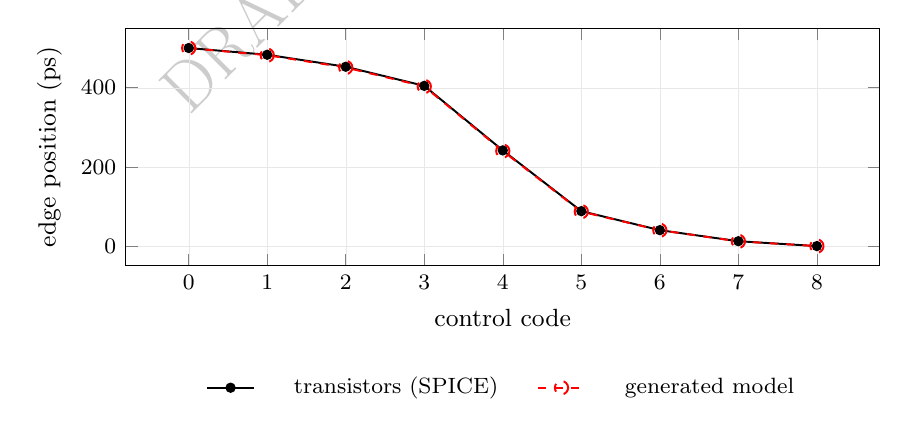
\begin{tikzpicture}
  \begin{axis}[width=0.92\linewidth,height=4.6cm,
    xlabel={control code}, ylabel={edge position (ps)},
    label style={font=\small}, tick label style={font=\footnotesize},
    legend style={font=\footnotesize,at={(0.5,-0.42)},anchor=north,
      legend columns=2,draw=none,column sep=1.2em},
    grid=both, grid style={line width=0.1pt,draw=gray!18},
    every axis plot/.append style={line width=0.7pt}]
    \addplot[black,mark=*,mark size=1.5pt] coordinates {(0,500.1) (1,483.12) (2,452.83) (3,404.61) (4,241.62) (5,88.23) (6,40.214) (7,12.363) (8,0)};
    \addplot[red,dashed,mark=o,mark size=2.4pt] coordinates {(0,500) (1,482) (2,451) (3,403) (4,240) (5,87) (6,40) (7,12) (8,0)};
    \legend{transistors (SPICE), generated model}
  \end{axis}
\end{tikzpicture}
\end{center}
\vspace{-0.6em}
\noindent{\footnotesize Nine codes, nine measured answers. There is no waveform to compare here: what the block does is place an edge, so that is what is plotted.}\vspace{0.6em}
% <<END TRACE:pi>>

%======================================================================
\section{Case study 4 --- Phase-locked loop}

The first three are single blocks. This one is a \emph{loop}, and that
changes what a model has to get right. In a loop, a small error does not
stay small --- it is fed back around and pushes the whole system to a
different operating point. So a model that looks perfectly reasonable on
its own can still settle the loop somewhere the real circuit never goes.

It is also three different characterisation problems in one netlist, and
no single method covers them. The pipeline classifies each block from its
topology and routes it accordingly:

\begin{center}
\begin{tabular}{@{}lll@{}}
\toprule
\textbf{Block} & \textbf{Why the default does not fit} & \textbf{Route taken} \\
\midrule
\texttt{ro\_vco} & oscillates with its inputs at DC ---
                   & tuning curve, \\
                 & its output is a frequency, not a gain
                   & scored on rate \\
\texttt{cpump}   & a complementary pair driven from
                   & one $I(V)$ table \\
                 & independently controlled gates
                   & per control state \\
\texttt{lpfilt}  & only R and C, so its state space is
                   & exact state space, \\
                 & exact and needs no fitting
                   & read from topology \\
\bottomrule
\end{tabular}
\end{center}

\noindent Not one of those three is a simple input-to-output response. A
conventional flow that fitted one to each would be fitting the wrong
quantity three times over.

\subsection{Checked as a system, against the transistors}

A score for each block on its own is evidence about that block on its own.
A loop asks a different question: wired together, do these models behave
like the circuit? The co-simulation answers it directly. The design's own
testbench is run twice: once where the analog half is the generated
models, once where it is the real transistors through ngspice. Only the
small piece of code that connects the two halves is swapped between
runs. The thresholds, the expressions and the pass/fail logic are
byte-for-byte identical in both, so the two logs can be compared
line against line.

\begin{center}
\begin{tabular}{@{}lr@{}}
\toprule
Blocks modelled, three routes        & $3$ composed, $2$ more emitted \\
Per-block equivalence                & $5$ of $5$ pass \\
\midrule
Supply condition                     & $20\unit{mV}$ rms, declared in the deck \\
System check vs transistors          & $4$ boundary signals, $0$ failed \\
\quad \texttt{vout} (control voltage) & $1.86\unit{mV}$, bar $0.190$ \\
\quad \texttt{aout} (VCO output)      & $0.4\%$ of crossings, bar $2\%$ \\
\quad \texttt{dra} (internal probe)   & $8.96\unit{mV}$ \\
\midrule
Both loops lock at                   & $400.00\unit{MHz}$ \\
\quad settled control band           & $1.8468$--$1.8546\unit{V}$ vs \\
                                     & $1.8468$--$1.8499\unit{V}$ \\
\midrule
Model half vs transistor half        & $6.37\unit{s}$ vs $111.1\unit{s}$ \\
\quad same testbench, same span       & $17.4\times$ \\
\bottomrule
\end{tabular}
\end{center}

\noindent The control voltage is the number to read. It is where the loop
stores its state, so a model that settles anywhere else disagrees here
first --- and the two agree to $1.86\unit{mV}$ while reaching the same
frequency, on a rail carrying $20\unit{mV}$ rms of noise the deck
declares. That is looser than the figure this table carried while the
rail was quiet, and the rail is the reason: a loop concentrates a supply
disturbance onto precisely this node. Running the case that way is the
point of it.

% <<TRACE:pll>>
\begin{center}
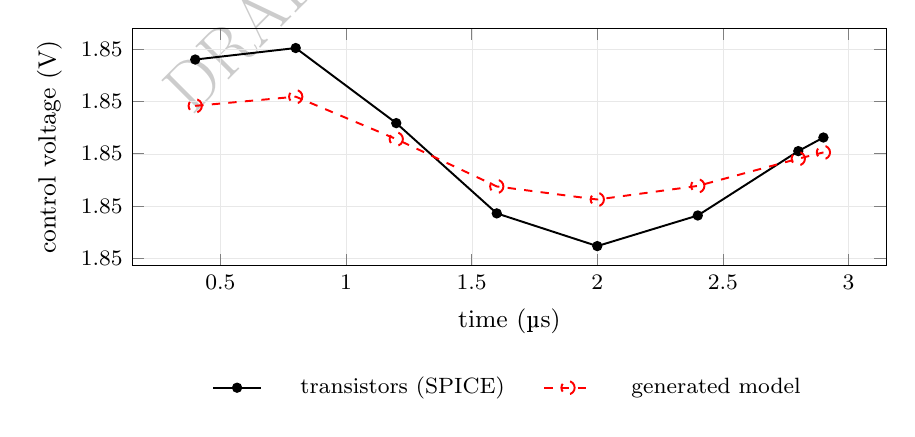
\begin{tikzpicture}
  \begin{axis}[width=0.92\linewidth,height=4.6cm,
    xlabel={time (\textmu s)}, ylabel={control voltage (V)},
    label style={font=\small}, tick label style={font=\footnotesize},
    legend style={font=\footnotesize,at={(0.5,-0.42)},anchor=north,
      legend columns=2,draw=none,column sep=1.2em},
    grid=both, grid style={line width=0.1pt,draw=gray!18},
    every axis plot/.append style={line width=0.7pt}]
    \addplot[black,mark=*,mark size=1.5pt] coordinates {(0.3999,1.8536) (0.7999,1.85404) (1.2,1.85117) (1.6,1.84772) (2,1.84647) (2.4,1.84764) (2.8,1.8501) (2.9,1.85062)};
    \addplot[red,dashed,mark=o,mark size=2.4pt] coordinates {(0.3999,1.85183) (0.7999,1.85218) (1.2,1.85056) (1.6,1.84875) (2,1.84825) (2.4,1.84877) (2.8,1.84981) (2.9,1.85005)};
    \legend{transistors (SPICE), generated model}
  \end{axis}
\end{tikzpicture}
\end{center}
\vspace{-0.6em}
\noindent{\footnotesize The control voltage at the co-simulation boundary: the composed models against the transistors, on the design's own testbench. The two track each other to within 1.9\,mV on a node the loop holds near 1.85\,V. Eight samples because that is how often the digital side reads this node.}\vspace{0.6em}
% <<END TRACE:pll>>

\textbf{That figure is one draw, and the bar beside it is not.} Both
halves generate their own noise from the declared source, so a
worst-window difference is a sample rather than a property of the model:
five consecutive runs of this same deck gave $3.61$, $1.83$, $4.15$,
$2.05$ and $1.86\unit{mV}$ here. What does not move is what the
difference is judged against --- $0.190$ of \texttt{vout}'s own scale, of
which $0.140$ is the allowance for exactly this sampling --- and that is the number the
verdict is against and the record carries. An agreement figure quoted
without its bar tells you less than it seems to, in the same way as a
jitter ratio quoted without its correlation time.

Each node also records which of its two metrics that bar governs. A
node the digital side consumes through a threshold is judged on its
crossings, not on its mean. Printing the mean beside the crossing bar
would read as a pass against a bar it exceeded: $0.030$ against $0.020$,
where the number actually compared was $0.004$.

\subsection{The rail the deck declares is the rail the model sees}
\label{sec:noise}

The netlist for this case says

\begin{center}
\texttt{vdd dd 0 dc \{vcc\} trnoise(0.02 1e-10 0 0)}
\end{center}

\noindent --- a supply with $20\unit{mV}$ rms on it, redrawn every
$100\unit{ps}$. A composition that reads that line and emits
\texttt{assign dd\_v = 3.3;} has deleted a disturbance the design asked
for, and every check downstream then agrees about a circuit nobody is
shipping. A transient of this deck puts that source at
$10.91\unit{ps}$ rms of period jitter at the oscillator, $\pm 5\%$ at the
two hundred cycles it was measured over. That figure is itself a draw. A
constant rail produces none of it.

That figure is measured per design rather than quoted. Getting it
needs one step first: the declared condition is restored onto the block's
own supply. Extraction rebuilds every rail as a plain DC source, so the
fragment a block is characterised from does not carry the noise its
design states. Without that step the measurement would be of a quieter
circuit than the one being modelled. The generated file says which source
the number came from.

So the declared source is carried into the composed model, sampled and
held at the source's own interval. That reproduces the two properties
which decide how much jitter a source causes --- its rms and its
correlation time. The spectra agree at low frequency and part near
$1/NT$, where ngspice interpolates between its noise breakpoints and the
model does not.

\textbf{All seven fields of a \texttt{trnoise} declaration are read}, not
the white pair alone. Where a deck declares flicker, the composition
carries it as a Voss--McCartney summation across the octaves the run
spans; where it declares a random telegraph, as a two-state Markov
process with exponentially distributed dwells, at the capture and
emission times given. The Voss construction produces $\alpha = 1$, and
the generated file records both that and the exponent the deck asked for
rather than quietly substituting one for the other. This PLL declares the
white pair alone, which is why every figure here is white --- 1/f is what
dominates close-in phase noise, and a deck that states it gets it.

Carrying it changes what a comparison means. Both halves now draw their
own noise, so two runs of the same circuit differ by sampling error
alone and a fixed tolerance would be measuring run length. Each node's
bar is widened by three standard errors of the difference between two
window means, taken from the reference's own spread rather than from the
declared amplitude --- what actually reaches a node is a property of the
circuit. On \texttt{vout} that allowance is $0.140$ of the $0.190$ bar,
and the record carries both, so a reader can see how much of the bar was
earned and how much was allowed.

\subsection{Where the block works is measured, not assumed}

The two output-buffer inverters sit in the clock path. Their job is to
place edges in time, and an average voltage error is close to blind to
that. Both pass an average-error comparison comfortably --- while their
error at the single worst instant is $99.9\%$ of the full voltage swing.
Those are not in conflict: if the model's edge lands slightly late, then
for that brief moment the model sits at one supply rail while the real
circuit sits at the other. Averaged over time it vanishes. For a clock
buffer, that moment is the behaviour being verified. The pipeline
classifies them from the measured DC curve --- $62\%$ and $61\%$ of
swept points within $5\%$ of a rail is a switching characteristic, not a
smooth response --- and scores them on duty cycle instead.

The frequency it scores them at is measured. Where a block operates is a
property of the closed loop and exists only once the digital side is
attached, exactly like the operating range the golden probe already
measures. The probe therefore measures each net's switching rate beside
its voltage band: the two inverter inputs return $399.8$ and
$399.7\unit{MHz}$, the $400\unit{MHz}$ this PLL locks to. Scored there,
they pass at $0.276$ and $0.307\unit{pp}$ of duty against a
$0.5\unit{pp}$ bar.

The form they are re-emitted in has no delay line, so it cannot carry the
measured rise/fall skew --- $0.589$ and $0.672\unit{pp}$ of duty at that
clock. Both blocks measure below their own floor, so the skew partly
cancels rather than adding. That makes the floor an upper bound on what
the form costs, not margin to spend, and the pipeline states it before
scoring rather than leaving a pass to be read as unqualified.

That number is not one a language model can supply. Asked five times
about the same inverter with the same measurements, the classifier
proposed clock rates of $2\unit{MHz}$, $765\unit{MHz}$, $300\unit{MHz}$,
$10\unit{GHz}$ and $15\unit{GHz}$; asked about the second stage, it
proposed $10\unit{GHz}$. The lowest is two hundred times below where the
buffer runs and the highest thirty-seven times above what its own model
can follow. The measurement returns the same answer every run, and gives
the two stages answers agreeing to $0.03\%$, which no classifier run did.
Intent from the model, physics from the circuit, applied to a number that
looked like intent and was not.

What the classifier is asked for, it has been steady on: buffer, clock
stimulus, duty metric, on every run of both stages. That is the judgement
gated on a measurement it can check itself against. What moved is the one
number it was in no position to know.

\paragraph{The verdict names the metric it came from.}
Asking for the classifier is not the same as getting it. Every duty
figure above comes from a run with a key present and the classifier
consulted. The same demonstration was then run deliberately
\emph{without} one, to see what a reader would be shown if it declined.
The chirp is kept, and these same two blocks pass an rms comparison at
$0.025$ against a $0.15$ bar --- a green result from a measurement that
cannot see the property in question. The two transcripts are otherwise alike, and the
command line is identical, so the run records which figure each verdict
was reached by, and the demonstration reports it from that record.
Asking for a check on the command line does not show that it ran.

%======================================================================
\section{Results at a glance}

\begin{center}
\begin{tabular}{@{}llrr@{}}
\toprule
\textbf{Case study} & \textbf{Environment} & \textbf{Checks} & \textbf{Failed} \\
\midrule
Filter        & DC $+$ AC                  & $49 + 15$ & $0$ \\
Duty corrector & DC $+$ duty               & $46 + 14$ & $0$ \\
Phase interpolator & phase per code        & $9$       & $0$ \\
Phase-locked loop & co-simulation vs transistors & $5 + 4$   & $0$ \\
\bottomrule
\end{tabular}
\end{center}

\noindent The first three case studies --- characterisation, model
generation, both simulators, and every generated environment --- run end
to end in under $16$ minutes on a laptop. The PLL is a further
$15$ minutes, most of it the ring oscillator's tuning curve.

All four are one command, and \texttt{demo\_4\_pll.sh} runs this one.
It differs from the others in what it needs, not in how it is run. Being
the analog half of a co-simulation, it needs the other half: the RTL, the
DPI bridge, and a \emph{shared} libngspice --- a different ngspice build
from the binary the first three use. It checks for each of those before
doing any work and names what is missing. A machine without them gets a
skip saying which piece and where it comes from, rather than a failure
twelve minutes into a run. spice2rnm's outputs are
simulator-agnostic: plain IEEE 1800 SystemVerilog, tied to no vendor. So
that anyone can reproduce the results here, all of them were produced
with open-source simulators --- \textbf{ngspice} for characterisation and
the reference transients, \textbf{xezim} for both the transient
equivalence co-simulation and the generated UVM-MS environments. No commercial licence was used anywhere in this
document. The generated artifacts themselves are published for
inspection: the models, the complete environments, and the evidence
files, exactly as the tool wrote them. They are at

\begin{center}
\url{https://github.com/vrajeshprakhya/spice2rnm-demos}
\end{center}

\noindent under \texttt{showcase/}, stamped with the tool version and run
summary that produced them. What the repository holds:

\begin{lstlisting}
spice2rnm-demos/
  README.md          what this repository is, and is not
  .gitignore         run scratch; the showcase is curated, not
                     whatever a run left behind
  demo_1_lpf.sh  demo_2_dcc.sh  demo_3_pi.sh
  demo_4_pll.sh  run_all.sh
                     the four case studies, runnable end to end
  harness/           8 measurement scripts the demos call
  showcase/          the generated artifacts, byte-for-byte
    lpf2/            the baseline case, 14 files + equivalence/:
      rc_lpf2_rnm.sv          the model, plain real ports
      rc_lpf2_rnm_wreal.sv    the same model, wreal ports
      rc_lpf2_ms_types_pkg.sv nettype real rc_lpf2_wire,
                              resolved by summing its drivers
      rc_lpf2_dms.sv          net <-> variable, interconnect ports
      rc_lpf2_bridge*.sv      MS bridge and its driving core
      rc_lpf2_proxy_pkg.sv    agent <-> bridge API
      rc_lpf2_ms_pkg.sv       agent, and the SPICE goldens
      rc_lpf2_ms_scoreboard.svh  the checks and tolerances
      rc_lpf2_ms_tb/test.svh  environment and test
      top_rc_lpf2_ms.sv       nets, DUT, bridge, test
      run_rc_lpf2_ms.sh       compiles and runs it
      result.json             fit, verdict, warnings
      equivalence/            what the check actually ran and found
    dcc2/            same shape, 15 files + equivalence/: no AC
                     section, adds duty goldens in dcc_ms_pkg.sv
                     and the run log pipeline.txt
    pi/              same shape, 14 files + equivalence/: an MS
                     bridge, proxy and agent like the others, with
                     phase-per-code goldens and no DC or AC section
    pll/             50 files + equivalence/: five block models, three
                     interfaces, the composed analog top, the
                     node package, result.json, and env/ --
                     three per-block UVM-MS environments plus
                     the SYSTEM one, where the design's own RTL
                     and every block's model elaborate together,
                     carrying a period-jitter monitor at 1 fs
    house_lib/       4 files, NOT generated: ng_ams_pkg.sv
                     declaring nettype real ng_anet, and two
                     hand-written models using it
    lpf2_house/      13 files: lpf2 again, joined to house_lib --
                     no types package, and rc_lpf2_rnm_ng_anet.sv
                     in place of the wreal boundary
    STAMP            date, tool version, and run summary that
                     produced the artifacts above
    refresh.sh       regenerates everything; the only way this
                     directory is ever updated
  whitepaper/        this document, source and PDF
\end{lstlisting}

\subsection{What the equivalence folders hold}

Every case study publishes an \texttt{equivalence/} directory: what the
check ran, what it found, and a manifest of what was left out.

\begin{center}
\begin{tabular}{@{}lll@{}}
\toprule
\textbf{Case} & \textbf{Judged on} & \textbf{Published verdict} \\
\midrule
Filter        & rms voltage        & $0.0290$ against $0.15$ \\
Duty corrector & rms voltage       & $0.0769$ against $0.15$ \\
Phase interpolator & phase per code & worst $1.832\unit{ps}$ at code 2, \\
              &                    & tolerance $6.251\unit{ps}$ \\
Phase-locked loop & five routes, then & five block verdicts, and the \\
              & the whole system   & system over $116{,}018$ samples \\
\bottomrule
\end{tabular}
\end{center}

\noindent Each folder carries three things. \texttt{verdict.txt} is
lifted from that run's own \texttt{result.json} rather than retyped, so a
number here cannot disagree with the run that produced it. The simulator
and SPICE logs say what actually executed. And the comparison table gives
one row per measured point. The phase interpolator's
\texttt{phase\_compare.csv} is nine rows, one per control code, with the
measured delay, the model's delay and the error. The PLL's
\texttt{rc\_compare.csv} is the loop filter's response to an injected
current, sample by sample.

\paragraph{What is manifested rather than published, and why.}
The waveform routes write one row per simulator timestep rather than one
per measured point, so the filter's aligned comparison is
$18.6\unit{MB}$ and its generated testbench $18\unit{MB}$; the duty
corrector's waveform dump is $11.7\unit{MB}$. Around $80\unit{MB}$ across
four cases, in a repository whose history is permanent, for files
\texttt{refresh.sh} regenerates in half an hour. Every one is named in
\texttt{MANIFEST.txt} with its exact size and the command that recreates
it, so a reader sees what exists and what it weighs without every future
clone carrying it. What is published comes to $232\unit{kB}$.

The distinction is drawn by size rather than by filename. A
comparison table small enough to read is evidence; one large enough to be
a waveform is a trace. The routes differ in which they produce --- a
network compared point by point writes a table, a waveform compared
sample by sample writes a trace --- so the rule has to be about the file,
not about what it is called.

\noindent And what it deliberately does not hold: the spice2rnm tool
itself (the product is licensed separately; this repository is its
evidence), and the build products of the runs --- characterisation
scratch, compiled simulator objects, DPI shims. \texttt{refresh.sh}
filters those out, so the showcase is what a user would keep, not
everything a run produces.

%======================================================================
\section{What the equivalence check compares}
\label{sec:equiv}

Every model in this document was checked the same way. The generated
SystemVerilog is loaded into a digital simulator and fed an input signal.
The transistor circuit is fed the very same input in SPICE. The two
outputs are then lined up in time and compared point by point, and both
traces are saved, so anyone can go back to the run's own folder and work
out the number again for themselves.

Two things about that arrangement matter more than the numbers it
produces. The first is that \textbf{it reads the file you are actually
handed}. There is a weaker number some tools report --- how well the
fitted maths matched its own measurements. That number never opens the
generated file, and would look identical if the file had been written out
wrongly. This check loads that file into a simulator and runs it, so a
code-generation bug fails it.

The second is that \textbf{each block is scored on its own job}. One error
figure used everywhere would be blind on most of these blocks: an average
voltage error cannot see where an edge lands, and a frequency has no
voltage error to measure in the first place.

\begin{center}
\begin{tabular}{@{}lll@{}}
\toprule
\textbf{If the block} & \textbf{then compare} & \textbf{and score it as} \\
\midrule
passes a signal   & the output waveform, on    & the error, against how \\
through           & a sweep and on a second,   & far the output itself \\
                  & unrelated input            & moves \\[0.3em]
drives a clock    & where the edges land, at   & duty error, in \\
                  & the rate measured in use   & percentage points \\[0.3em]
moves an edge     & the crossing time at       & picoseconds, plus step \\
per setting       & every setting              & size and evenness \\[0.3em]
oscillates        & the output frequency, as   & a percentage of that \\
                  & the control voltage varies & frequency \\[0.3em]
switches a        & the current it drives, in  & a percentage, for each \\
current           & each switch position       & position \\[0.3em]
is passive R/C    & the output's response to   & the error, against how \\
                  & a current pushed into it   & far the output moves \\
\bottomrule
\end{tabular}
\end{center}

\noindent Every verdict records which of these rows it came from. Months
later, a reader can still tell which number actually decided the result
from the numbers that were merely noted alongside it.

\subsection{What keeps a figure from flattering itself}

\textbf{Some measurements are held back.} Where a block is characterised
by measuring it at many points, a share of those points is kept out of the
model-building and used only for scoring. The headline figure is then not
the fit marking its own work. The charge pump in case study 4 reports
$0.549\%$ held back; the ring oscillator reports its held-back frequency
error directly.

\textbf{An input the model has never seen.} The filter in case study 1 is
built from a frequency sweep and then tested with a pseudo-random bit
sequence it was never shown ($0.0097$). A model that had merely memorised
what it was built from is exposed there.

\textbf{The report says what range the answer covers.} A comparison proves
nothing about conditions it never drove, so the report states the range it
did drive. The ring oscillator is the clearest case, and the honest answer
there is two numbers. Inside the voltage band the loop actually operates
in, its held-back frequency error is $0.002\%$. At the far edge of the
wider range that was characterised --- where the curve bends hardest, and
where the loop never goes --- it reaches $4.99\%$. Both are reported. The
verdict is taken in the band that matters, and the less flattering number
is printed rather than quietly dropped.

\textbf{What the model shape cannot do is priced in advance.} Sometimes
the shape of model chosen simply cannot represent something the circuit
does. When that happens, the cost is stated up front, in the same units as
the verdict --- as with the inverter timing asymmetry in case study 4,
quoted as duty error at the clock rate in use. A pass is then read against
that floor, instead of being taken as a clean win.

\subsection{Blocks, and then the system}

The table above scores blocks one at a time. Putting blocks together asks
a further question, because errors that are small individually need not
stay small once everything is wired up. Two levels of check answer it.

The first needs nothing but the netlist. The assembled model is driven at
the outside edge of the design, and its output is compared against the
full transistor circuit driven the same way.

The second applies when what you hand the tool is a co-simulation --- a
design whose analog half already talks to a digital half --- and it is the
one case study 4 reports. Here the design's own testbench is run twice.
Once, the analog half is the generated models. Once, it is the real
transistors. Everything else is left alone: the digital logic, the limits
it checks against, and the pass/fail rules are byte-for-byte identical in
both runs, and only the small piece of code joining the two halves is
swapped. That makes the two runs directly comparable, signal by signal:
$4$ signals crossing between the halves, $0$ failed, the control voltage
agreeing to $4.15\unit{mV}$ on a rail carrying $20\unit{mV}$ rms of
declared noise, and both versions locking to the same frequency.

And a check that does not apply to a given run is reported as not
applicable, with the reason why. It is never quietly counted as a pass.

\subsection{One thing a score at an operating point cannot see}
\label{sec:jitter}

Every check described so far is \emph{static}: it compares a value at an
operating point. That is the right shape for most of what a model claims,
and it is blind to one error that matters.

An oscillator model has to decide when to place its next edge. One way
reads the control voltage at the instant the previous edge fired and
schedules a whole half cycle from it. Another integrates the control
across the cycle, which is what the circuit does. Both models carry the
\emph{same} tuning curve, so a check that measures frequency at held
control voltages scores them identically --- and it does: run against
both, it passes both. Give them the same moving control and they part: on
the reference ring, fed a control with a $100\unit{ps}$ correlation time,
the sampling form produced $3.37\times$ the period jitter the transistors
did.

How far apart they land is not a fixed property of the two forms. It is
$\sqrt{T_{\mathrm{half}}/\tau}$ in the correlation time $\tau$ of the
disturbance, which for $1.25\unit{ns}$ against $100\unit{ps}$ predicts
$3.54$ --- the measurement above, to within $5\%$. A faster disturbance
separates them further, so a ratio quoted without its $\tau$ says less
than it appears to.

So the tool checks the dynamic behaviour directly. A known disturbance is
injected in SPICE at several amplitudes, and the disturbance
\emph{ngspice actually solved} is replayed into the model sample for
sample. That last part is the point: giving the model its own random
noise of the same size would compare two random sequences, and agreement
between those says more about how long the run was than about the model.
Replaying the same waveform compares transfer.

Both of the model's inputs are exercised, not just the obvious one. On the
reference ring the supply moves the frequency by $450.6\unit{MHz/V}$,
comparable to the control port and opposite in sign, so a model given no
supply input cannot show what a droop does at all. The verdict is the
worse of the two paths.

\begin{center}
\small
\begin{tabular}{llrrr}
\hline
\textbf{Path} & \textbf{Injected} & \textbf{Circuit} & \textbf{Model} & \textbf{Ratio}\\
\hline
either  & none (floor)      & $0.051\unit{ps}$  & $0.000\unit{ps}$  & not judged\\
\hline
control & $5\unit{mV}$ rms  & $2.396\unit{ps}$  & $2.352\unit{ps}$  & $0.981$\\
        & $20\unit{mV}$ rms & $8.743\unit{ps}$  & $8.690\unit{ps}$  & $0.994$\\
        & $50\unit{mV}$ rms & $26.719\unit{ps}$ & $25.618\unit{ps}$ & $0.959$\\
\hline
supply  & $5\unit{mV}$ rms  & $2.808\unit{ps}$  & $2.640\unit{ps}$  & $0.940$\\
        & $20\unit{mV}$ rms & $11.617\unit{ps}$ & $12.139\unit{ps}$ & $1.045$\\
        & $50\unit{mV}$ rms & $28.422\unit{ps}$ & $27.656\unit{ps}$ & $0.973$\\
\hline
\end{tabular}
\end{center}

These ratios are a draw, like the boundary figures earlier. Each
injection is a fresh realisation and an rms over two hundred cycles
carries about $5\%$ on each side, so the same six points on the previous
run read $0.987$, $0.946$, $0.925$ and $0.896$, $0.953$, $0.970$. That
spread is why the bar is $0.25$ rather than something that looks
stricter: a tolerance tighter than the measurement's own uncertainty
fails correct models at a rate set by run length.

The floor row is measured and deliberately not judged. With nothing
injected the reference still reports about $54\unit{fs}$, which is how
precisely the edge-finder can locate a crossing rather than anything the
circuit did. Asking the model to reproduce it would be asking it to
reproduce an artefact. It is used instead as the floor every other
amplitude has to clear before its result counts.

That agreement was not obtained by fitting anything. Take the supply
path, where the sensitivity is separately measured: $450.6\unit{MHz/V}$ on a $2.509\unit{ns}$ period
predicts $14.18\unit{ps}$ of period jitter for $5\unit{mV}$ rms, if the
disturbance held still across the cycle. The circuit gives
$2.797\unit{ps}$ --- a ratio of $0.197$, against the
$\sqrt{\tau/T} = \sqrt{100.3\unit{ps}/2509\unit{ps}} = 0.200$ that
averaging over the cycle predicts.

It holds across the decade rather than at one point: $0.197$, $0.223$ and
$0.203$ at the three judged amplitudes, where an oscillator that did not
average its input would sit at $1$ --- five times higher. Three points
within $12\%$ of a parameter-free prediction, over a tenfold range, and
each carrying the same few per cent of sampling uncertainty as the
ratios above. The model reproduces it because
it integrates, and the version that samples does not.

\textbf{And it decides for itself whether the check is worth running},
because for most designs the honest answer is no and a quarter of an hour
is a real cost. Two things can say yes.

The first is the design's own closed-loop behaviour, measured: how far the
control moves within one oscillator period, carried through the tuning
curve's own slope into period movement, against what the reference
measurement can resolve. On this PLL it says no, and says it with numbers
--- on a run where it was the deciding voice, $12.18\unit{\textmu V}$ rms
per $2.503\unit{ns}$ period, worth $0.0288\unit{ps}$ against a
$0.0521\unit{ps}$ floor, $0.55\times$ what the reference can resolve. A
loop filter holds its control still; that is what a loop filter is for.

The second is the netlist, and it is what runs the sweep above: this deck
declares $20\unit{mV}$ rms on the ring's supply, and a design that writes
noise into its own deck is asking for noise to be simulated. That rule is
matched on the NET rather than the source name. Block extraction rebuilds
every supply as a plain DC source: the fragment carries
\texttt{VBIAS2 dd 0 DC 3.3} where the top level wrote
\texttt{vdd dd 0 dc \{vcc\} trnoise(...)}. The net survives and the source
name does not, so matched on the name the rule was unreachable on every
hierarchical run: on every run, that is, which has a top-level deck to
declare anything in.

There is no flag to force it, because a request to run a check is not
evidence that one is warranted. And where the tool has no closed-loop
evidence either way, it runs the check rather than skipping it: having no
opinion about whether a check is needed is not the same as deciding it is
not.

\paragraph{What the sweep measures, and what it does not.} The ring in
isolation, driven on its own characterisation fragment. That is the right
scope for the question it answers --- does this model transfer a
disturbance correctly --- and it is not the same question as what the
loop does with one. Inside the loop the filter holds the control still,
which is precisely why the closed-loop half of the gate declines; these
numbers come from driving the block directly, where nothing is holding
it. A reader should not read the supply column as a statement about this
PLL's supply rejection. It is a statement about the model.

%======================================================================
\section{Why a green testbench is worth believing}

Generated verification has an obvious credibility problem. If the same
tool writes the model \emph{and} writes the test, what stops it from
writing a test its own model is bound to pass? Three rules answer that.

\textbf{The right answers come from SPICE, never from the model.} Every
expected value in every generated environment is a SPICE measurement of
your circuit. Checking a model against the equations that model itself
implements would pass no matter how wrong the model was, so spice2rnm
never does it.

\textbf{Every environment is proven able to fail.} The tool deliberately
breaks the generated model and confirms the test goes red. It also
\emph{measures} how small a break it can still catch, rather than simply
claiming one. For the duty-cycle corrector's environment:

\begin{center}
\begin{tabular}{@{}ll@{}}
\toprule
\textbf{Injected fault} & \textbf{Detected by} \\
\midrule
comparator offset, $20\unit{mV}$   & DC and duty sections \\
dynamics slowed $10\times$         & duty section (DC is structurally blind) \\
dynamics slowed $50\times$         & duty section (DC is structurally blind) \\
\bottomrule
\end{tabular}
\end{center}

\noindent The right-hand column is the point. A DC check looks at the
circuit after it has settled, and that is the whole of what many
hand-written environments test. It cannot see \emph{any} error in how fast
a block responds --- slow this model down fiftyfold and the DC check still
passes it. The function-matched sections exist because of that blind spot,
and the fault sweep is re-run against the shipped model so these detection
claims stay true rather than becoming folklore.

\textbf{The test is checked in both directions.} A test that fails
everything is as useless as one that passes everything. So the same sweep
also confirms that errors small enough to be acceptable do \emph{not} trip
the environment.

%======================================================================
\section{Functional specifications as input}
\label{sec:spec}

A netlist says what a circuit \emph{is}. It never says what it is
\emph{for}, what rate it must run at, or how close is close enough. Hand
those to the tool as a plain-language document --- a datasheet excerpt, a
requirements page --- and it reads out the facts that shape verification:

\begin{center}
\begin{tabular}{@{}ll@{}}
\toprule
\textbf{From the specification} & \textbf{Used for} \\
\midrule
operating clock range          & where the environment drives the block \\
accepted input duty range      & the stimulus sweep \\
duty accuracy requirement      & the pass/fail tolerance \\
block function                 & which environment is generated \\
\bottomrule
\end{tabular}
\end{center}

\noindent On the duty-cycle corrector, the specification-driven run checks
$35$--$65\%$ input duty at the specified clock rates against the
specification's own $1.0$ pp requirement: $15$ checks, $0$ failed, worst
$0.428$ pp. \pass

\textbf{The specification is cross-checked, never trusted.} Every
extracted fact is validated against what the circuit was actually measured
to do, and the measurement wins. When the two disagree, that disagreement
is surfaced as a finding:

\begin{lstlisting}
SPEC CONFLICT: the spec says this block operates up to 4e+08 Hz, but
the fitted model is only valid below 1.195e+08 Hz -- 3.3x lower.
\end{lstlisting}

\noindent That is a coverage gap between a requirement and a
characterisation, caught at model-generation time instead of at silicon
correlation --- and it is the kind of finding no amount of manual model
review produces, because no one document contains both halves of it.

%======================================================================
\section{Joining an existing model library}
\label{sec:style}

A team with real-number models already has conventions --- which
user-defined nettype analog values travel on, which package declares it,
what discipline their model ports use. Generated files that import their
own freshly-invented nettype do not join that library; they sit beside it,
each net scheme blind to the other, and the integration cost lands on the
customer.

Point \texttt{-{}-style-from} at the library and the output conforms: the
environment's analog nets use \emph{their} nettype, its files import
\emph{their} package, no types package of the tool's own is emitted, and
the generated run script compiles their package file. A library whose
models use \texttt{wreal} ports gets the wreal wrapper without being
asked. Their timescale is reported but deliberately not adopted ---
generated delays are computed femtosecond values, and timescale is per
compilation unit, so the directives interoperate unchanged.

\textbf{Reading a house style is a judgement, so it is read and then
verified.} A library may declare several nettypes, only one of which is
the living standard --- and what says so is often a comment. Measured on a
library that declares two, where the deprecated one happens to sort first
alphabetically:

\begin{center}
\begin{tabular}{@{}ll@{}}
\toprule
mechanical scan & picks the deprecated nettype, and warns \\
model reading   & picks the live one, quoting the deprecation notice \\
verification    & re-checks the choice against the named file \\
\bottomrule
\end{tabular}
\end{center}

\noindent The model's stated grounds, verbatim from that run: \emph{``line
15 marks \texttt{aaa{}\_legacy{}\_wire} deprecated (``kept only so ancient
testbenches still compile. Do NOT use in new code\,''), \ldots{} both models
declare all analog ports as \texttt{acme{}\_ewire}, confirming this is the
live convention.''} Nothing in that reading is taken on trust: the named
nettype, package and file are checked against the file before use, and a
claim the file does not support leaves the mechanical answer standing,
out loud. Where the tool has a \emph{measurement} --- a count of which
discipline the library's ports actually use --- the count wins outright
and a disagreement is recorded rather than adopted.

\textbf{The result is an environment that runs on the house net},
and it is published rather than described. The showcase carries the same
filter twice: \texttt{lpf2/} generated normally, and
\texttt{lpf2{}\_house/} generated against
\texttt{house{}\_lib/} --- a small hand-written library standing in for a
customer's own. Diffing the two directories is the whole argument:

\begin{center}
\begin{tabular}{@{}lll@{}}
\toprule
 & \textbf{\texttt{lpf2/}} & \textbf{\texttt{lpf2{}\_house/}} \\
\midrule
types package & emitted            & \textbf{not emitted} \\
nets          & \texttt{rc{}\_lpf2{}\_wire} & \texttt{ng{}\_anet} \\
imports       & the generated one  & \texttt{ng{}\_ams{}\_pkg} \\
run script    & compiles it        & compiles the house package \\
model ports   & plain \texttt{real}     & \texttt{ng{}\_anet}, and the
                                     environment instantiates it \\
\midrule
the model     & \multicolumn{2}{l}{byte-identical} \\
the scoreboard & \multicolumn{2}{l}{byte-identical} \\
\bottomrule
\end{tabular}
\end{center}

\noindent Conformance changes the boundary and nothing else --- and the
published environment runs from where it sits, against the library beside
it: $49$ DC and $15$ AC checks, $0$ failed, exactly the default
environment's result.

Note what the environment instantiates in that second column. When the
model is delivered behind a port boundary, the generated testbench drives
\emph{that} module rather than the core inside it, and the boundary's
file joins the compile list --- so what the evidence covers is what
ships, not a component of it. Measured separately, a library resolving its net by
averaging rather than summing conforms and passes the same way, and a
library using \texttt{wreal} ports gets the wreal wrapper instead.
Without \texttt{-{}-style-from}, or against a directory with nothing
recognisable in it, nothing changes --- and the run says so.

\section{AI where it helps, physics where it decides}

spice2rnm asks a language model four kinds of question: where one block
ends and the next begins, what a block is for, what a written
specification requires, and what conventions an existing model library
follows (Section~\ref{sec:style}). Every one of those is a question of
\emph{intent}. None is a question of physics.

That is the rule the tool works by: \textbf{intent from the model, physics
from the measurement}. Every suggestion is checked against the measured
circuit before it is used. One that does not check out is discarded, the
run carries on with what was measured, and it says that it did so. With no
API key at all, every AI feature declines cleanly and the pipeline runs
entirely on measurement.

Which of those two happened is recorded in the run's own result, not only
in its log. A verdict carries the metric it was reached by. A report
read months later can then tell a check that ran from one that declined
and fell back. Without that, every green result would have to be taken on
trust that the feature requested was the feature exercised.

%======================================================================
\section{Scope and requirements}

\begin{itemize}[leftmargin=1.5em,itemsep=0.3em]
  \item \textbf{Inputs}: SPICE netlists, flat or with subcircuits;
        optional plain-language functional specification; optionally an
        existing RNM library to take conventions from.
  \item \textbf{Outputs}: SystemVerilog real-number models, with the
        port discipline of your choice --- plain \texttt{real} (portable
        anywhere), \texttt{wreal}, or your library's own nettype; UVM-MS 1.0
        environments; equivalence reports with archived waveforms.
  \item \textbf{Toolchain}: a SPICE simulator for characterisation,
        and a digital simulator capable of running real number models ---
        with UVM support for the generated environments. The generated
        models and environments are standard SystemVerilog and carry no
        vendor dependence, so either may be the one your flow already
        uses.
  \item \textbf{Block-level scope}: single-input single-output blocks and
        compositions of them, including current-mode blocks sharing a
        node. Hierarchical composition trades some accuracy for structure;
        the equivalence report states the composed figure separately from
        the per-block figures, so the trade is visible, not hidden.
  \item \textbf{Jitter TRANSFER is verified; intrinsic device noise is
        characterised.} Both are measured, and they are measured
        differently.

        What is checked is what the model does with a disturbance it is
        given: injected in SPICE, replayed into the model, period jitter
        compared, on both the control and the supply. Section~%
        \ref{sec:jitter} gives the measurements --- six judged points over
        a tenfold range, worst ratio $0.940$ against a $0.25$ tolerance,
        reached by the pipeline's own decision because the deck declares
        noise on a net the ring is wired to. This is a real check with a
        verdict, and it fails a model whose transfer is wrong.

        The oscillator's own noise is characterised through its
        impulse sensitivity function, which the pipeline measures without
        being asked: a narrow charge injected at each phase of the cycle,
        the lasting phase shift measured, and $\Gamma(\phi)$ is the
        sensitivity that results.\footnote{%
        The method is Hajimiri, Limotyrakis and Lee, \emph{Jitter and
        Phase Noise in Ring Oscillators}, IEEE JSSC 34(6), June 1999. Two
        details decide whether it works, and each returns a plausible
        wrong answer rather than an error, so the tool enforces both. The
        pulse is applied differentially where the circuit is differential
        --- into one node of a differential ring it is mostly common
        mode, which the ring rejects by design, and the measurement then
        reads its own floor however large the pulse. And linearity is
        judged at the phase of greatest sensitivity rather than a
        convenient one: the same charge that moves the phase by
        $0.04\unit{ps}$ where the ring barely responds moves it by
        $52\unit{ps}$ at the peak.}
        On the reference ring $\Gamma_{\mathrm{rms}}$ is
        $4.04\times10^{12}\unit{rad/C}$ from the automated sweep, against
        $4.33\times10^{12}$ measured by hand: the two agree to $7\%$.
        $\Gamma$ changes sign across the cycle as a ring's must, and
        halves when the injected charge halves.

        $\Gamma_{\mathrm{rms}}$ times a device noise density is a jitter:
        $0.236$ to $0.578\unit{ps}$ rms here, or $-114.5$ to
        $-106.7\unit{dBc/Hz}$ at $1\unit{MHz}$, reported as a range
        because the channel-noise factor and the way per-node densities
        combine are both ranges. The model carries it as a parameter,
        shipped at zero: the figure is computed from the measured ISF
        rather than compared against a reference transient, since ngspice
        simulates no device noise in one.

        \textbf{Driven blocks jitter differently, and the models say so.}
        An oscillator measures each edge from its own last one, so its
        phase random-walks and the error accumulates. A buffer or a lag
        block measures its output from an \emph{input} event, so every
        traversal draws independently and nothing accumulates.\footnote{%
        The distinction and both implementations are Kundert's, in
        \emph{Modeling and Simulation of Jitter in Phase-Locked Loops},
        AACD 1997. He makes four points this model follows. Driven
        systems jitter without accumulating; autonomous ones have a phase
        difference that is ``a random walk that is not bounded''. The
        metric for both is $J = \sigma(T)$, the standard deviation of one
        period. Driven jitter is modelled by ``randomly dithering the
        delay argument \ldots{} on every output transition''. And the
        per-update dither scales by $\sqrt{N}$ for $N$ updates per
        period, which is $1.414$ for the two this model uses.

        Each was checked. Asked for $1\%$ rms period jitter, the model
        produced $0.9998\%$. Its scaling constant is the $\sqrt{2}$ his
        listing specifies. And over $30{,}000$ cycles, the variance of
        the accumulated deviation grew linearly in cycle count, at
        $1.004 \pm 0.026$ of the $k J^2$ his random walk requires.

        The check also found a defect. At one sub-step per half cycle the
        scheduler cannot resolve a randomised threshold. The model now
        refuses that combination, rather than reporting $39.6\%$ jitter
        where $1\%$ was asked.} The
        scheduled-lag models take a synchronous-jitter figure on that
        basis, perturbing the input-to-output delay once per traversal.
        That figure is supplied, not measured: a transient of a deck
        declaring no noise has no delay variation in it to measure. The
        generated file says so. It also states the constant latency the
        perturbation costs, because a tap only looks backwards, so an
        edge can be early only relative to a delay already present.

        Edge JITTER is measured where the reference has edges. On the
        reference PLL's two clock-path buffers it is $3.98\unit{ps}$ and
        $3.60\unit{ps}$, reported beside the skew because the two fail
        differently. It is reported rather than judged: there is no
        threshold for it, and inventing one from a single design would be
        worse than showing the number. The system equivalence check does
        not judge it either, and the reason is the probe rather than
        the model. Its boundary log is sampled at $100\unit{ps}$. The
        composed model's output crosses its threshold between samples, so
        a crossing can only be located to the nearest tick. Reporting
        that as jitter would be measuring the sampling grid.

        The generated UVM-MS environment carries a monitor without that
        limitation. It is event-driven on the signal rather than sampled
        on a clock, and compiled at \texttt{1fs} while the rest of the
        environment stays at \texttt{1ps}, which costs nothing anywhere
        else because SystemVerilog scopes timescale per module. Running
        that environment on the composed PLL gives $12.70\unit{ps}$ rms
        of period jitter over $1151$ periods at the boundary, with none
        of its system checks failed and one inconclusive, over
        $116{,}012$ boundary crossings. The number of checks is not
        quoted because it is not fixed: one of them exists only where the
        transistor reference settled measurably, which under a noisy rail
        it may or may not do.

        REPORTED, NOT JUDGED, and for a specific reason rather than
        caution. A loop
        suppresses its oscillator's jitter inside the loop bandwidth, so
        a figure measured at the boundary is not the block's own jitter
        and the two are not expected to agree. The $10.91\unit{ps}$ this
        deck's declared rail is worth at \texttt{ro\_vco} is a different
        measurement of a different quantity. On this run they differ by
        $16\%$; on the one before, by $3\%$. Both are draws, and neither
        is evidence about the other.

        This is further than published practice goes on the validation
        side, while the gap named above --- intrinsic noise in the model
        --- is one the same practice also has. Analog Devices'
        production RNM suite for a GHz transceiver validates its PLL on
        lock time and frequency error, the same quantities checked in
        Section~\ref{sec:equiv}. It states that ``model validation
        remains an area for improvement in the real number modeling
        flow'', and names frequency-domain performance as future
        work.\footnote{J.~Dudek, \emph{Real Number Modeling of RF
        Circuits}, DVCon. The paper notes that because RNMs exist to
        enable system-level testing, ``the requirements for model
        validation are greatly relaxed in this environment''.}
\end{itemize}

\vspace{1.5em}
\noindent\rule{\linewidth}{0.4pt}
\vspace{0.3em}

\noindent{\footnotesize \textcopyright{} 2026 Veylon Systems.
spice2rnm is a Veylon Systems product. Every figure in this document was
produced by the shipped tool from its bundled demonstration circuits, most
recently on 2026-09-16. The demonstration suite at
\url{https://github.com/vrajeshprakhya/spice2rnm-demos} regenerates them
in one command.}

\end{document}
